\documentclass[degree=bachelor, tocarialchapter]{bnuthesis}
% 选项
%   degree=[bachelor|master|doctor|postdoctor], % 必选,学位类型
%   secret,                % 可选(默认:关闭),是否有密级
%   tocarialchapter,       % 可选(默认:关闭),章目录中使用黑体(这项表示同时打开下面两项)
%   tocarialchapterentry,  % 可选(默认:关闭),单独控制章标题在目录中使用黑体
%   tocarialchapterpage,   % 可选(默认:关闭),单独控制章页码在目录中使用黑体
%   pifootnote,            % 可选(默认:关闭),页脚编号采用 pifont 字体符号,建议打开

% 所有其它可能用到的包都统一放到这里了,可以根据自己的实际添加或者删除。
\usepackage{bnuthesis}



% 定义所有的图片文件在 figures 子目录下
\graphicspath{{figures/}}

% 可以在这里修改配置文件中的定义。导言区可以使用中文。
% \def\myname{薛瑞尼}

\begin{document}

%%% 封面部分
\frontmatter
\bnusetup{
  %******************************
  % 注意:
  %   1. 配置里面不要出现空行
  %   2. 不需要的配置信息可以删除
  %******************************
  %
  %=====
  % 中文信息
  %=========
  ctitle={等温捷径与绝热捷径构成的类卡诺循环热机的功率与效率},
  cdegree={理学学士},
  cdepartment={物理学系},
  cmajor={物理学},
  cauthor={龚政楠},
  csupervisor={涂展春~教授},
  cassosupervisor={涂展春~教授}, % 校内
  % 日期自动使用当前时间,若需指定按如下方式修改:
  %=========
  % 英文信息
  %=========
  etitle={Finite Time Thermodynamics},
  edegree={Bacholar of Science},
  emajor={Physics},
  eauthor={R.Z},
  esupervisor={XXX},
  eassosupervisor={XXXX},
  % 日期自动生成,若需指定按如下方式修改:
  % edate={December, 2005}
  %
  % 关键词用“英文逗号”分割
  ckeywords={有限时间热力学, 等温捷径, 绝热捷径, 类卡诺热机},
  ekeywords={TeX, LaTeX, CJK, template, thesis}
}

% 定义中英文摘要和关键字
\begin{cabstract}
  论文的摘要是对论文研究内容和成果的高度概括。摘要应对论文所研究的问题及其研究目
  的进行描述,对研究方法和过程进行简单介绍,对研究成果和所得结论进行概括。摘要应
  具有独立性和自明性,其内容应包含与论文全文同等量的主要信息。使读者即使不阅读全
  文,通过摘要就能了解论文的总体内容和主要成果。

  论文摘要的书写应力求精确、简明。切忌写成对论文书写内容进行提要的形式,尤其要避
  免“第 1 章……;第 2 章……;……”这种或类似的陈述方式。

  本文介绍清华大学论文模板 \bnuthesis{} 的使用方法。本模板符合学校的本科、硕士、
  博士论文格式要求。

  本文的创新点主要有:
  \begin{itemize}
    \item 用例子来解释模板的使用方法;
    \item 用废话来填充无关紧要的部分;
    \item 一边学习摸索一边编写新代码。
  \end{itemize}

  关键词是为了文献标引工作、用以表示全文主要内容信息的单词或术语。关键词不超过 5
  个,每个关键词中间用分号分隔。(模板作者注:关键词分隔符不用考虑,模板会自动处
  理。英文关键词同理。)
\end{cabstract}

% 如果习惯关键字跟在摘要文字后面,可以用直接命令来设置,如下:
% \ckeywords{\TeX, \LaTeX, CJK, 模板, 论文}

\begin{eabstract}
   An abstract of a dissertation is a summary and extraction of research work
   and contributions. Included in an abstract should be description of research
   topic and research objective, brief introduction to methodology and research
   process, and summarization of conclusion and contributions of the
   research. An abstract should be characterized by independence and clarity and
   carry identical information with the dissertation. It should be such that the
   general idea and major contributions of the dissertation are conveyed without
   reading the dissertation.

   An abstract should be concise and to the point. It is a misunderstanding to
   make an abstract an outline of the dissertation and words ``the first
   chapter'', ``the second chapter'' and the like should be avoided in the
   abstract.

   Key words are terms used in a dissertation for indexing, reflecting core
   information of the dissertation. An abstract may contain a maximum of 5 key
   words, with semi-colons used in between to separate one another.
\end{eabstract}

% \ekeywords{\TeX, \LaTeX, CJK, template, thesis}
% 如果使用授权说明扫描页,将可选参数中指定为扫描得到的 PDF 文件名,例如:
% \makecover[scan-auth.pdf]
\makecover
 
%% 目录
\tableofcontents

%% 符号对照表
\begin{denotation}[3cm]
  \item[$m$] 质量。本篇文章只涉及一种粒子,为简单令$m\equiv1$
  \item[$k_\M{B}$] 玻尔兹曼常数,$1.380649 \times 10^{−23}\ \M{J/K}$。为了方便,令$k_\M{B}\equiv1$
  \item[$N_{\mathrm{A}}$] 阿伏伽德罗常数,$6.02 \times 10^{23}$    
  \item[$h$] 普朗克常量,$6.62607015 \times 10^{-34}\  \M{J \cdot s}$
  \item[$\hbar$] 约化普朗克常量,$\hbar \equiv \frac{h}{2\pi}$
\end{denotation}
 


%%% 正文部分
\mainmatter
\chapter{绪论:从经典热力学到随机热力学}
\label{c1}
热机的发明和使用对人类的生产生活产生了重大的影响,第一次工业革命和第二次工业革命都和热机的发展有紧密的关系。 一直以来,特别是近些年来,由于能源短缺的问题愈发突出,研究热机的效率问题也一直吸引着一大批研究者。

\section{引言:热机的最大功率与效率问题}
\qquad 早在1824,卡诺(Sadi Carnot)就指出(基于热质说)\cite{2005}:工作在相同高温热源$T_{\M{h}}$和低温热源$T_{\M{c}}$的所有热机中,以可逆热机的效率最高,而且这些可逆热机的效率都相同,为$\eta _{\text{c}}=1-\frac{T_{\M{c}}}{T_{\M{h}}}$ 。这个问题似乎就这么解决了,然而必须注意的是卡诺热机要求循环过程是可逆的。也就是说,要想达到卡诺热机的效率,热机一个循环的工作时间应当是无限长,这样的热机功率为0。

我们当然不可能接受功率为0的热机,所以研究者开始关注热机在某一功率下(特别是最大功率)的最大效率,而这个问题促进了有限时间热力学的诞生。

1975年,Curzon和Ahlborn构建了了内可逆热机\cite{Curzon1975},该热机可在有限时间内完成一个循环。并且得到了该热机在最大功率下的效率为$\eta _{\mathrm{CA}}=1-\sqrt{T_{\mathrm{c}}/T_{\mathrm{h}}}=1-\sqrt{1-\eta _{\mathrm{c}}}$ ,其中$\eta _{\mathrm{c}}$为卡诺效率。

2008年,T. Schmiedl 和 U. Seifert提出了微观随机热机模型\cite{Schmiedl2008},该热机模型利用依赖于时间的谐振子势场驱动布朗粒子做功,并得到了其在最大功率下的效率:$\eta_{\M{TU}}={ \eta_{0}}/{(2-\eta_{0}/2)}$

同年,涂展春推导出费曼棘轮热机\cite{Tu2008}在最大功率下的效率$\eta _{\text{F}}=\frac{\eta _{\text{C}}^{2}}{\eta _{\text{C}}-\left( 1-\eta _{\text{C}} \right) \ln \left( 1-\eta _{\text{C}} \right)}$。 \cite{Tu2020}

……



同时涂展春\cite{Tu2008}在小温差条件下,即$\eta _{\text{c}}\rightarrow 0$。 将上述热机的效率按照 展开. 发现这些效率到二阶项都相同的,它们都普遍地满足$\eta _{\text{U}}=\frac{\eta _{\text{c}}}{2}+\frac{\eta _{\text{c}}^{2}}{8}+O\left( \eta _{\text{c}}^{3} \right)$。 这个规律在其他热机中也得到了验证,但也有一些热机不满足这个关系. 这引发了研究者对相关问题的思考,涂展春在紧耦合热机的范畴内对其中的原因进行了解释.\cite{Tu2020}

在这些形形色色的有限时间热机中,由Seifert等人提出的微观随机热机\cite{Schmiedl2008}占据一席之地. 随机热机通常是利用外势驱动粒子对外做功. 其中的具体的实现过程可以有很大的不同,对应着不同类型的随机热机。2014年,Campo等人利用绝热捷径构建了奥托热机\cite{DelCampo2014}。 而后,Deng等人发现绝热捷径能够提高奥托热机的效率,不论是经典的还是量子的情形下。\cite{Deng2013} 2014年,涂展春在Schmiedl和Seifert工作\cite{Schmiedl2008}的基础上,考虑了他们在过阻尼情况下忽略的粒子的惯性的影响,构建了一种类卡诺热机\cite{Tu2013},并且惊讶地发现这种随机热机的效率等于Curzon和Ahlborn构建的内可逆热机\cite{Curzon1975}的效率。在涂展春构建的热机中,布朗粒子在与时间相关的谐振子$U=\lambda ^2\left( t \right) q^2/2$的控制下,经历了类卡诺循环. 其中与卡诺循环中绝热过程对应的就是前面提到的绝热捷径,但与卡诺循环中等温过程对应的“等温过程”,却只是粒子与恒温热源接触,而非系统保持恒温..

这促使我们思考是否有与卡诺循环中等温过程更加对应的过程来实现类卡诺循环过程。等温捷径\cite{Li2016}的提出为实现这个目标提供了契机,李耿等人给一个系统引入了辅助势,这个系统的演化本来是被一个含时哈密顿量所决定的,这个精心选择的辅助势可以使得系统在当前的哈密顿量下的状态,仿佛处于原哈密顿量的瞬时平衡态中一样,从而实现了“等温过程”,他称之为等温捷径.

于是,我们意欲构造一种由绝热捷径和等温捷径构成的类卡诺循环热机,并且根据随机热力学中的典型方法,研究该热机工作过程中的效率与功率。 与其他类型的热机,如涂展春构建的类卡诺热机\cite{Tu2013},Campo等人构建的奥托热机\cite{DelCampo2014}进行比较。
\section{经典热力学}

\qquad 经典热力学是从宏观的角度研究物质的。它所用的概念,如温度、密度、压强等,都是物质的宏观属性。这些都是不以物质的原子结构为基础就可以定义的概念。再根据宏观的观察和分析得到关于这些概念的经验性的规律和关系,经典热力学就是这样得以发展的。这些经验性的规律和关系被延伸为四个基本定律,即所谓的热力学第零定律、第一定律、第二定律、第三定律,以这些定律为基础就构成了经典热力学。热力学原理(及其基本定律)具有相当的普遍性,即它们不依赖于任何有关物质结构的特殊假设,因为它们根本不以物质的微观特性为基础。由于这种普遍性,热力学的应用范围非常广泛。以至于爱因斯坦说道\cite{schilpp1979albert}:“(热力学)是唯一普遍适用的物理理论,我确信,在这个理论的基本概念适用的范围内,它绝不会被推翻。”\footnote{It is the only physical theory of universal content, which I am convinced, that within the framework of applicability of its basic concepts will never be
overthrown.}

\subsection{经典热力学简史}

\qquad 经典热力学的历史最早可以追溯到克里克(Otto von Guericke),他在1650年建造和设计了世界上第一台真空泵,并借此演示了著名的马德堡半球实验(Magdeburg hemispheres)。Guericke的实验推翻亚里士多德(Aristotle)长期以来的假设,即 "大自然厌恶真空"。之后不久,英裔爱尔兰物理学家和化学家波义耳(Robert Boyle)得知了Guericke的设计,并在1656年与英国科学家胡克(Robert Hooke)合作,制造了一个气泵。\cite{partington1989short} 利用这个气泵,Boyle和Hooke注意到了压力、温度和体积之间的关系。随着时间的推移,\textbf{波义耳定律(Boyle's Law)}被发现,该定律指出:温度相同时,气体压力和体积成反比。

时间来到1824年,这一年“热力学之父”卡诺发表了\textit{Reflections on the Motive Power of Fire} (《关于火的动力的思考》),论述了热、功率、能量和热机效率。该书概述了卡诺热机、卡诺循环和动力之间的基本能量关系。它标志着热力学作为一门现代科学的开始。\cite{perrot1998z}

随后在19世纪50年代,热力学第一定律和第二定律被提出,主要出自威廉·兰金(William Rankine)、克劳修斯(Rudolf Clausius)和开尔文(William Thomson)的著作。接着,统计热力学的基础由麦克斯韦(James Clerk Maxwell)、玻尔兹曼(Ludwig Boltzmann)、普朗克、克劳修斯和吉布斯(J.Willard Gibbs)等物理学家建立。

1873-76年间,吉布斯发表了一系列的三篇论文,最著名的是\textit{ On the Equilibrium of Heterogeneous Substances}(《论异质物质的平衡》)\cite{connecticut1866transactions},他在论文中说明了如何利用图像分析包括化学反应在内的热力学过程,通过研究热力学系统的能量、熵、体积、温度和压力,可以确定一个过程是否会自发发生。\cite{sugi1993scientific} 另外,19世纪的杜赫姆(Pierre Duhem)也写了关于化学热力学的文章\cite{duhem1886potentiel}。 20世纪初,吉尔伯特·N·刘易斯(Gilbert N. Lewis)、梅尔·兰德尔(Merle Randall)\cite{lewis1923thermodynamics}和E·A·古根海姆(E. A. Guggenheim)\cite{guggenheim2002modern,guggenheim1967advanced}等化学家将吉布斯的方法应用到化学过程的分析中。从中也可以窥见热力学的适用性之广。

\subsection{经典热力学的基本概念}
\qquad 按爱因斯坦的说法,在热力学的基本概念适用范围内,热力学本身也是适用的。这一方面说明了热力学概念的运用之宽泛,另一方面也说明爱因斯坦并没有将热力学的适用范围无限扩大。不管如何,这都说明了热力学中的这些概念的重要性。而且现在,其中很大一部分概念已经渗透进其他学科、社会和生活的方方面面。
\begin{itemize}
    \item 系统\cite{Wu2010}:泛指个体的集合,这些个体之间通常有相互作用。在经典热力学中,一个系统通常指宏观系统,其包含的基本个体数的量级为$N_{\mathrm{A}}$。不与外界相互作用,包括不进行物质交换和热交换等的系统被称为\textbf{孤立系统}。
    \item 平衡态:在没有外界影响的条件下,如果一个系统的的状态不随时间变换,没有力学的、化学的变化和热传递,我们称这个系统达到了热力学平衡态。
    \item 态函数:对于一个处于热力学平衡态的系统,有若干的宏观性质,这些性质可以用宏观的量加以描述。比如\textbf{温度}、\textbf{体积}、\textbf{压强}、\textbf{自由能}、\textbf{焓}、\textbf{内能}、\textbf{熵},注意这些态函数并不都是独立的。
    \item 内能:内能是系统的态函数,可以看做系统所包含全部个体的平均动能和相互作用势能之和
    \item 熵:熵是系统的态函数,它和热力学第二定律息息相关。大概是热力学中最具影响力的概念,已经成为科学衡量无序和信息的基本标尺,在社会学中也有一定的应用。\cite{rifkin1980entropy}
\end{itemize}

\subsection{热力学基本定律}
\qquad 如前所述,热力学建立在四个基本定律之上。对于具体的系统,具体的问题,通常还要在加上一些唯象的假设,才能够解决相应的问题。
\begin{itemize}
    \item 热力学第零定律:如两个系统之间达到了热平衡态,则两个系统必有一相同的态函数。这个态函数其实就是温度。\cite{Wu2010}热力学第零定律也常常被叙述为:如果两个系统分别与第三个系统达到热平衡态,则这两个系统之间也达到了热平衡态。
    \item 热力学第一定律:热力学第一定律描述了能量在转换与转移过程中的守恒。设一个系统从外界吸收热量$Q$,外界对它做功$W$,内能增加$\Delta U$,则必有$\Delta U = Q + W$。这个定律是由经验而来的,因为所有妄图无中生有产生能量的企图都宣告失败。
    \item 热力学第二定律:第一定律对能量的转化和转移过程除了作了守恒限制外,并没有做其他限制。但就经验来看,有些过程虽然没有违反第一定律,但依然不可能发生。根据这些,我们可提炼出热力学第二定律,它说明系统演化的方向性。热力学第二定律有很多不同的等价的表述方式,如克劳修斯表述:热量不能自发的从低温物体传递到高温物
    体;开尔文表述:不可能从单一热源中吸收热量,并全部用来做功,而不产生其他影响。\cite{Wang2013}

    根据热力学第二定律可以定义系统的一个态函数——熵,两个平衡态的熵差定义为$\Delta S = S_{A} - S_{B} = \int_{A}^{B} \frac{\dbar Q{\mathrm{rev}}}{T}$,其中下标rev代表可逆过程。根据熵的定义,由热力学第二定律可以证明孤立系统的熵永不减少,即$\md S \ge 0$。这也是热力学第二定律的数学表述。

    到19世纪末50年代,在由Maxwell和Boltzmann等人建立的统计热力学中,给予了熵以微观的理解——系统的无序度。按此观点,热力学第二定律是一个概率性的定律。
    \item 热力学第三定律:一个凝聚系统,在可逆等温过程中的熵变,在热力学温度$T$趋近于$0$时也趋近于零。第三定律有如下著名推论:不可能通过有限步骤使一个物体的温度达到热力学零度。有了热力学第三定律我们就可以把系统的熵确切的定义出来\cite{Wang2013},而不是只定义熵变。
\end{itemize}

\section{随机热力学}
\qquad 经典热力学主要研究系统平衡态下的性质和平衡态间的转化,对于处于非平衡态下的系统的性质和不可逆过程中,经典热力学能回答我们的并不多。对于偏离平衡态不多的非平衡态的性质,在20世纪三四十年代,普里高津\cite{prigogine1965introduction}和德格鲁特\cite{de2013non}等人建立了线性不可逆热力学。它现在已经发展成为一个成熟的理论,也解决了非常多的非平衡态中的问题,比如温差电效应等。\cite{Wang2013}本文的重点并非线性不可逆热力学,在此不做介绍。

对于远离平衡态的情形,线性不可逆热力学依然无能为力。21世纪以来,生物科技和纳米技术的发展促进了人们对\textbf{小系统}的研究,与经典热力学研究的宏观系统不同,这种纳米尺度的小系统包含的粒子数要远小于$N_{\mathrm{A}}$。所以小系统的涨落效应和脱离平衡态的的程度都很大。1998年,Ken Sekimoto在研究用过阻尼郎之万方程描述的随机体系中,基于状态演化的随机相轨,给出了体系内能变化、输入功和吸收热等热力学变量的定义\cite{Sekimoto1998}。2005年,Udo Seifert进一步阐明,在受驱动布朗粒子中,体系的熵和熵产生同样可以基于单个随机相轨进行定义\cite{Seifert2005},至此随机热力学正式建立。它将经典热力学中的功、热和熵等概念扩展到了单个轨道的情形。下面我们以一维布朗粒子为例进行介绍。

\subsection{随机动力学}
\label{c1s3}
\qquad 根据牛顿第二定律,可以容易的写出处于一维势场中的布朗粒子的运动方程
\begin{equation}
    \frac{\md q}{\md t}=p, \quad \frac{\md p}{\md t}=-\frac{\partial U(q,\lambda)}{\partial q}-\gamma p+\xi(t)
    \label{eq1.1}
\end{equation}
这就是\textbf{郎之万方程(Langevin Equation)},其中$\gamma$是阻尼系数,$\xi(t)$是高斯白噪声。依赖于时间的势场$U(q,\lambda)$施加在布朗粒子上,$\lambda\equiv\lambda(t)$是外界控制的势场的参数。对于$\xi(t)$,我们有
\begin{equation}
    \left\langle\xi\left(t\right)\right\rangle_{\xi}=0,\quad \left\langle\xi\left(t_{1}\right) \xi\left(t_{2}\right)\right\rangle_{\xi}=2 \gamma T  \delta\left(t_{2}-t_{1}\right)
    \label{eq1.2}
\end{equation}
其中$\left\langle \cdots \right\rangle_{\xi}$是对随机变量$\xi(t)$的不同实现的平均,第二个式子等式右边的系数$2 \gamma T$是能量均分定理的要求。\cite{Reichl2016}

在本文中,我们更常用的是描述布朗粒子的另一个等价的方程——\textbf{福克-普朗克方程(Fokker–Planck Equation)}\cite{Reichl2016},福克-普朗克方程从另一个方面描述了布朗粒子,决定了布朗粒子的概率密度的演化。令$\rho_{\xi}(q,p,t)$为布朗粒子对于某一个随机力的实现$\xi(t)$的概率密度,而我们关心的实际上是$\rho(q,p,t)\equiv\langle \rho(q,p,t) \rangle_{\xi}$,即对随机力的实现$\xi(t)$的平均,这个量才是我们在实验中能够观测到的。它表明在实际情形下,我们在时刻$t$,位置$q+\md q$处找到动量为$p+\md p$的布朗粒子的概率为$\rho(q,p,t) \md q \md p$。福克-普朗克方程正是描述了这个量的演化。下面我们来从朗之万方程推导福克-普朗克方程

对于$\rho_{\xi}(q,p,t)$,有刘维尔定理(Liouville Theorem)\cite{Wang2013}
\begin{equation}
    \PP{\rho_{\xi}}{t} + \nabla \cdot \left(\rho_{\xi} \bm{v} \right)=0
    \label{eq1.3}
\end{equation}
其中$\bm{v}\equiv\left(\dot{q}\hat{\mathbf{q}} + \dot{p}\hat{\mathbf{p}}\right)$,算符$\nabla \equiv \hat{\mathbf{q}} \partial / \partial q+\hat{\mathbf{p}} \partial / \partial p$,$\hat{\mathbf{q}}$和$\hat{\mathbf{p}}$是单位方向向量。
将朗之万方程\eqref{eq1.1}代入上式\eqref{eq1.3}得到
\begin{equation}
    \frac{\partial \rho_{\xi}}{\partial t}=-\hat{L}_{0} \rho_{\xi}-\hat{L}_{1} \rho_{\xi}
    \label{eq1.4}
\end{equation}
其中微分算符$\hat{L}_{0}$和$\hat{L}_{1}$的定义为
\begin{equation}
    \hat{L}_{0}=p \frac{\partial}{\partial q}-{\gamma}-{\gamma} p \frac{\partial}{\partial p}-\frac{\partial U}{\partial q} \frac{\partial}{\partial p},\quad \hat{L}_{1}= \xi(t) \frac{\partial}{\partial p}
    \label{eq1.5}
\end{equation}

引入概率密度$\sigma(t)$,使得
\begin{equation}
    \rho_{\xi}=\mathrm{e}^{-\hat{L}_{0} t} \sigma
    \label{eq1.6}
\end{equation}
根据式\eqref{eq1.4}有
\begin{equation}
    \frac{\partial \sigma(t)}{\partial t}=-\hat{V}(t) \sigma(t)
    \label{eq1.7}
\end{equation}
其中$\hat{V}(t)=\mathrm{e}^{+\hat{L}_{0} t} \hat{L}_{1}(t) \mathrm{e}^{-\hat{L}_{0} t}$。方程\eqref{eq1.7}有形式解
\begin{equation}
    \sigma(t)=\exp \left(\int_{0}^{t} \mathrm{~d} t^{\prime} \hat{V}\left(t^{\prime}\right)\right) \sigma(0)
    \label{eq1.8}
\end{equation}
利用幂级数展开可将上式\eqref{eq1.8}写成
\begin{equation}
    \sigma(t)=\left[\sum_{n=0}^{\infty} \frac{(-1)^{n}}{n !}\left(\int_{0}^{t} \mathrm{~d} t^{\prime} \hat{V}\left(t^{\prime}\right)\right)^{n}\right] \sigma(0) .
    \label{eq1.9}
\end{equation}
现在我们取等式\eqref{eq1.9}两边的平均$\langle \cdots \rangle_{\xi}$。根据对高斯白噪声的Wick定理\cite{Reichl2016},幂级数将只留下偶次幂项
\begin{equation}
    \begin{split}
        \langle\sigma(t)\rangle_{\xi}&=\left[\sum_{n=0}^{\infty} \frac{1}{2 n !}\left\langle\left(\int_{0}^{t} \mathrm{~d} t^{\prime} \hat{V}\left(t^{\prime}\right)\right)^{2 n}\right\rangle_{\xi}\right] \sigma(0)\\
        &=\left[\sum_{n=0}^{\infty} \frac{1}{n !}\left(\frac{1}{2} \int_{0}^{t} \mathrm{~d} t_{2} \int_{0}^{t} \mathrm{~d} t_{1}\left\langle\hat{V}\left(t_{2}\right) \hat{V}\left(t_{1}\right)\right\rangle_{\xi}\right)^{n}\right] \sigma(0)\\
        &=\exp \left(\frac{1}{2} \int_{0}^{t} \mathrm{~d} t_{2} \int_{0}^{t} \mathrm{~d} t_{1}\left\langle\hat{V}\left(t_{2}\right) \hat{V}\left(t_{1}\right)\right\rangle_{\xi}\right) \sigma(0)
    \end{split}
    \label{eq1.10}
\end{equation}
现在来计算上式\eqref{eq1.10}中的积分
\begin{equation}
    \begin{split}
    &\frac{1}{2} \int_{0}^{t} \mathrm{d} t_{2} \int_{0}^{t} \mathrm{d} t_{1}\left\langle\hat{V}\left(t_{2}\right) \hat{V}\left(t_{1}\right)\right\rangle_{\xi} \\
    =&\gamma T \int_{0}^{t} \mathrm{d} t_{2} \int_{0}^{t} \mathrm{~d} t_{1} \delta\left(t_{2}-t_{1}\right) \mathrm{e}^{+\hat{L}_{0} t_{2}} \frac{\partial}{\partial p} \mathrm{e}^{-\hat{L}_{0}\left(t_{2}-t_{1}\right)} \frac{\partial}{\partial p} \mathrm{e}^{-\hat{L}_{0} t_{1}} \\
    =&\gamma T \int_{0}^{t} \mathrm{d} t_{1} \mathrm{e}^{+\hat{L}_{0} t_{1}} \frac{\partial^{2}}{\partial p^{2}} \mathrm{e}^{-\hat{L}_{0} t_{1}}   
    \end{split}
    \label{eq1.11}
\end{equation}
将上式\eqref{eq1.11}代入式\eqref{eq1.10},并对式\eqref{eq1.10}取对时间$t$的偏微分可得
\begin{equation}
    \frac{\partial\langle\sigma(t)\rangle_{\xi}}{\partial t}=\gamma T \mathrm{e}^{+\hat{L}_{0} t} \frac{\partial^{2}}{\partial p^{2}} \mathrm{e}^{-\hat{L}_{0} t}\langle\sigma(t)\rangle_{\xi}
    \label{eq1.12}
\end{equation}
有了这个结果,我们就能得到$\rho(q,p,t)$的运动方程,注意到$\rho=\langle\rho_{\xi}\rangle_{\xi}=\mathrm{e}^{-\hat{L}_{0} t} \langle\sigma\rangle_{\xi}$,于是不难得到
\begin{equation}
    \frac{\partial \rho}{\partial t}=-\hat{L}_{0}\rho+\mathrm{e}^{-\hat{L}_{0} t} \frac{\partial\langle\sigma(t)\rangle_{\xi}}{\partial t}=-\hat{L}_{0}\rho+\gamma T \frac{\partial^{2} \rho}{\partial p^{2}}
    \label{eq1.13}
\end{equation}
结合上式\eqref{eq1.13}和式\eqref{eq1.5}可以得到
\begin{equation}
    \frac{\partial \rho}{\partial t}=-v \frac{\partial \rho}{\partial q}+\frac{\partial}{\partial p}\left[\left({\gamma} v+ \PP{U}{q}\right) \rho\right]+\gamma T \frac{\partial^{2} \rho}{\partial p^{2}}
    \label{eq1.14}
\end{equation}
这就是福克-普朗克方程。很重要的是我们注意到福克-普朗克方程满足概率守恒,这一点将它写为连续性方程的形式就清楚了。
\begin{equation}
    \PP{\rho}{t} + \nabla \cdot \bm{J} = 0
\label{eq12.57}
\end{equation}
其中
\begin{equation}
\bm{J} \equiv \rho  p  \hat{\mathbf{q}}-\rho\left(\gamma p+\frac{\partial U}{\partial q} + \frac{\gamma}{\rho \beta} \frac{\partial \rho}{\partial p}\right) \hat{\mathbf{p}}
\label{eq12.57.5}
\end{equation}
算符$\nabla \equiv \hat{\mathbf{q}} \partial / \partial q+\hat{\mathbf{p}} \partial / \partial p$,$\hat{\mathbf{q}}$和$\hat{\mathbf{p}}$是单位方向向量。

对于阻尼很大的情况,即过阻尼情况,我们可以忽略惯性的影响得到过阻尼情况下的郎之万方程
\begin{equation}
    0=-\frac{\partial U}{\partial q}-\gamma \frac{\md q}{\md t}+\xi(t)
    \label{eq1.17}
\end{equation}
对应的也有过阻尼的福克-普朗克方程
\begin{equation}
    \frac{\partial \rho}{\partial t} + \frac{\partial J}{\partial q}=0,
    \label{eq2.45}
\end{equation}
其中
\begin{equation}
    J=-\frac{1}{\gamma} \left(\frac{\partial U}{\partial q} \rho+\frac{1}{\beta} \frac{\partial \rho}{\partial q}\right)
    \label{eq2.45.5}
\end{equation}
上面的郎之万方程和相应的福克-普朗克方程都有自己适用的时间尺度,欠阻尼郎之万方程\eqref{eq3.1}适用的时间尺度要远大于环境中分子碰撞的时间尺度而远小于惯性的弛豫时间尺度$\tau_{\mathrm{c}}\equiv1/\gamma$;过阻尼郎之万方程适用的时间尺度则要远大于$\tau_{\mathrm{c}}$。\cite{Sekimoto2010}这一点在第\ref{c3e2}节中计算欠阻尼类卡诺热机的效率时将起到重要作用。

\subsection{随机能量学}
\label{c1s1.3.2}
\qquad 现在我们考虑为布朗粒子定义和经典热力学中对应的\textbf{吸收热}、\textbf{输入功}和\textbf{能量差}。环境对布朗粒子施加的力为$-\gamma p + \xi(t)$,那么粒子对环境有反作用力$-(-\gamma p + \xi(t))$,对于布朗粒子的一个轨道,当粒子的位移为$\md q$时,其对环境做的功为$-(-\gamma p+\xi(t)) \circ \md q$\footnote{"$\circ$"表示Stratonovich类型的乘积,它允许我们使用常规的微分运算。\cite{Gardiner,Sekimoto2010}}从环境的角度看,环境向粒子传递了$(-\gamma p+\xi(t)) \circ \md q$的能量。Sekimoto将它\cite{Sekimoto1997,Sekimoto2010}定义为吸收热
\begin{equation}
    \dbar \bar{q} \equiv (-\gamma p+\xi(t)) \circ \md q
    \label{eq1.20}
\end{equation}
考虑到能量$e=\frac{1}{2}p^2 + U(q,\lambda)$,再结合郎之万方程\eqref{eq1.1},不难得到
\begin{equation}
    \begin{split}
        \dbar \bar{q} & \equiv\left(\frac{\md p}{\md t}+\frac{\partial U}{\partial q}\right) \circ \md q \\
        &=\frac{\md p}{\md t} \circ p \md t+\md U(q, \lambda)-\frac{\partial U}{\partial \lambda} \md \lambda \\
        &=\md\left(\frac{p^{2}}{2}\right)+d U(x, \lambda)-\frac{\partial U}{\partial \lambda} \md \lambda
    \end{split}
    \label{eq1.21}
\end{equation}
易得
\begin{equation}
    \md e=\md\left(\frac{p^{2}}{2}+U(q, \lambda)\right)=\dbar q+\frac{\partial U}{\partial \lambda} \md \lambda
    \label{eq1.22}
\end{equation}
结合经典热力学中的热力学第一定律,根据上式\eqref{eq1.22}我们可以定义输入功
\begin{equation}
    \dbar w \equiv \frac{\partial U}{\partial \lambda} \md \lambda
    \label{eq1.23}
\end{equation}

自此我们定义小系统中的热、功和能量差,这为我们讨论热机的功率和效率做好了准备。
\chapter{热机模型及绝热捷径和等温捷径}
\label{cha2}

\section{热机模型}
\qquad 本节我们将讨论几个典型的热机模型,它们中的每一个模型的提出对于相关领域都有重要价值。同时,回顾这几个热机模型的效率与功率的计算,也将为我们建立类卡诺热机模型和计算它的效率与功率提供思路。
\subsection{卡诺热机模型}
\qquad 卡诺热机对于热力学的意义大概怎么说都不算高估,正是基于卡诺的工作,克劳修斯和开尔文才提出了热力学第二定律。熵、绝对温标等重要的概念也是基于卡诺定理给出的。\cite{2005}

1824年,卡诺提出了卡诺热机模型如图\ref{f2.05},该热机由等温膨胀、绝热膨胀、等温压缩和绝热压缩四个可逆过程组成。
\begin{figure}[!htbp]
    \centering
    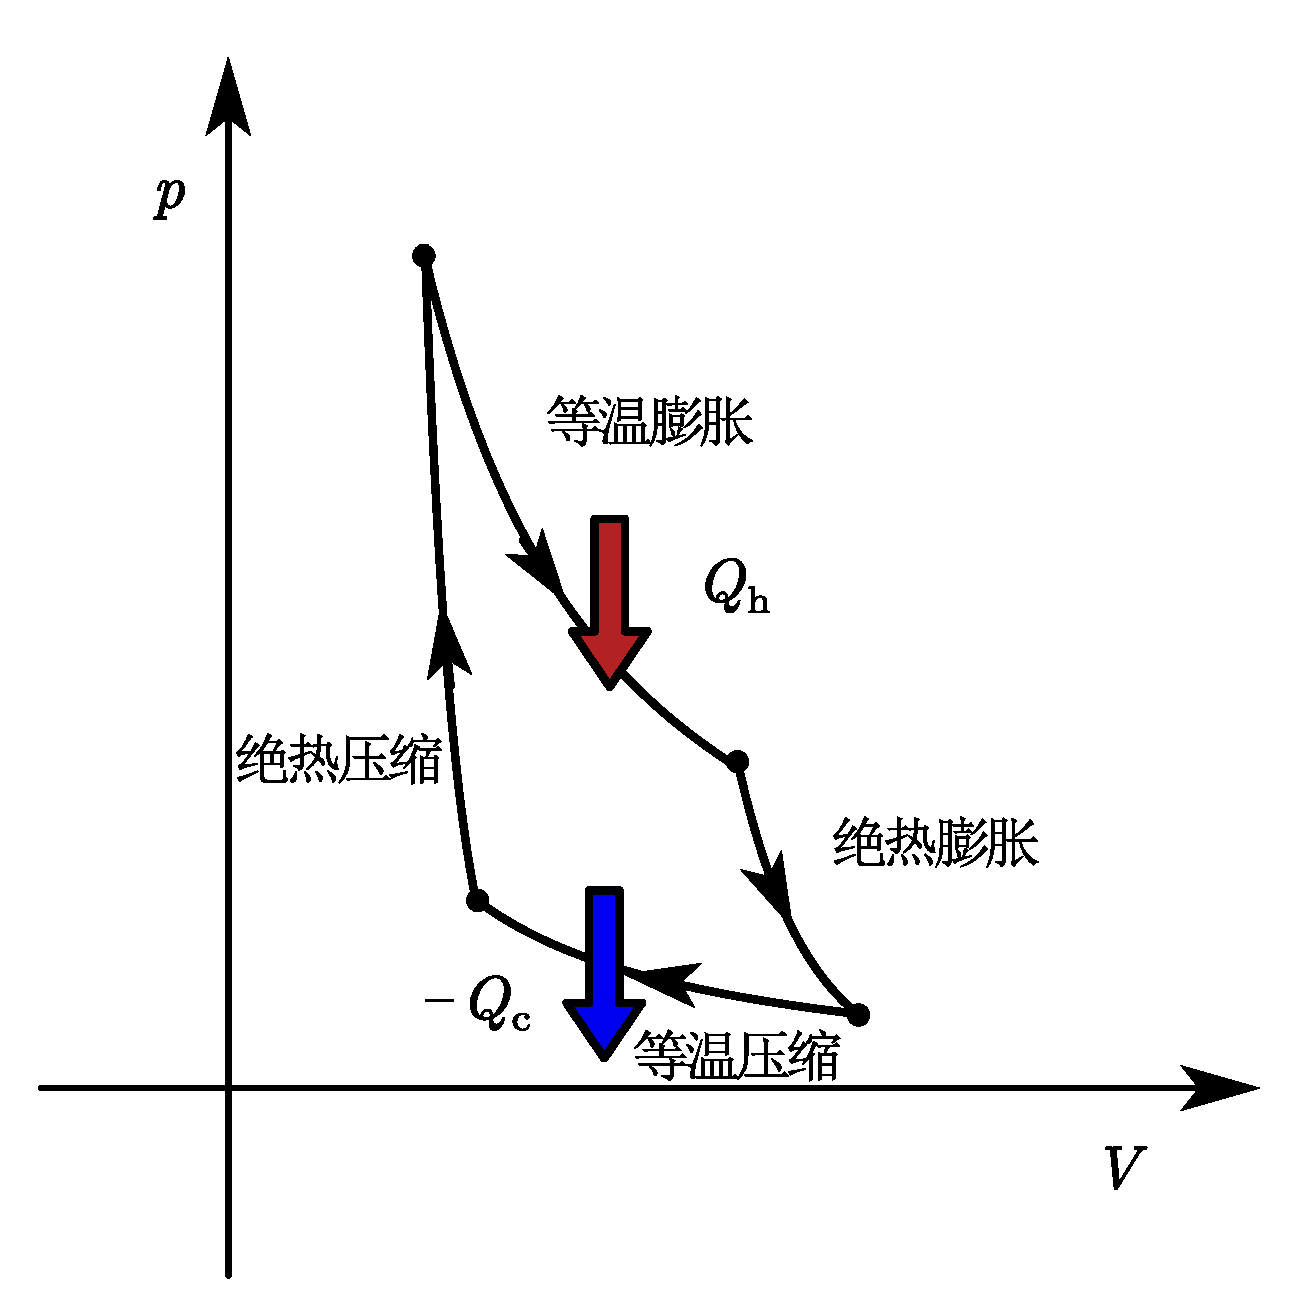
\includegraphics[width=0.4\textwidth]{p3.pdf}
    \caption{卡诺热机模型}
    \label{f2.05}
\end{figure}

热机的效率定义为$\eta\equiv\frac{-W}{Q_{\mathrm{h}}}$,$-W$是热机对外输出的功,$Q_{\mathrm{h}}$是热机从高温热源吸收的热。根据热力学第一定律,$-W=Q_{\mathrm{h}}+Q_{\mathrm{c}}$,其中$-Q_{\mathrm{c}}$是放给低温热源的热量。可得
\begin{equation}
    \eta=1+\frac{Q_{\mathrm{c}}}{Q_{\mathrm{h}}}
    \label{eq21.1}
\end{equation}
卡诺证明了卡诺热机的效率为
\begin{equation}
    \eta_{\mathrm{c}}=1-\frac{T_{\mathrm{c}}}{T_{\mathrm{c}}}
    \label{eq21.2}
\end{equation}
虽然卡诺热机在理论研究中有不可估量的价值,但在实际应用中却有不小的局限。问题在于卡诺热机是由可逆过程构成的,而可逆过程是无限缓慢的,那意味着卡诺热机的功率为0。所以虽然在所有工作在相同高温热源$T_{\mathrm{h}}$和低温热源$T_{\mathrm{c}}$的热机中以卡诺热机的效率为最大,但其功率却是最小的。上述功率与效率的矛盾促进了\textbf{有限时间热力学(FTT)}的发展
\subsection{内可逆热机模型}
\qquad 为了获得有限的功率输出,我们必须为卡诺热机中的可逆过程加速,这显然会导致效率的降低和不可逆熵的产生。有限时间热力学的专注点就是在有限时间内运行的热机的效率问题。而其中,一个重要而实际的议题就是热机在最大功率时的效率问题。

1975年,Curzon和Ahlborn提出了内可逆热机模型,\cite{Curzon1975}该热机可以在有限时间内完成一个循环。Curzon和Ahlborn内可逆热机(CA内可逆热机)的结构如图\ref{f2.06}所示。
\begin{figure}[!htbp]
    \centering
    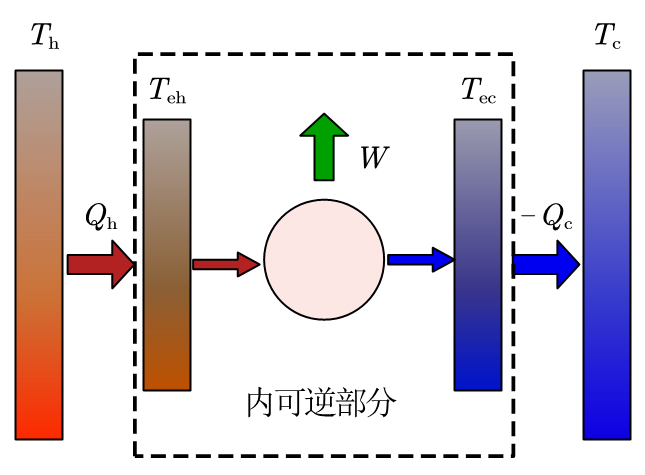
\includegraphics[width=0.4\textwidth]{p1.png}
    \caption{内可逆热机模型}
    \label{f2.06}
\end{figure}
CA内可逆热机是一种类卡洛热机,一个循环中也包含等温膨胀、绝热膨胀、等温压缩和绝热压缩这四个过程,不同之处在于它采用了四个假设
\begin{enumerate}
    \item 内可逆假设。假设等温膨胀和等温压缩过程中热机的温度并没有达到高温热源和低温热源的温度$T_{\mathrm{h}},\ T_{\mathrm{c}}$,而是达到了等效高温热源温度和低温热源温度$T_{\mathrm{eh}},\ T_{\mathrm{ec}}$。$(T_{\mathrm{h}}>T_{\mathrm{eh}}>T_{\mathrm{ec}}>T_{\mathrm{c}})$而且整个系统可以拆分为内可逆部分和外不可逆部分,鉴于内可逆部分不可逆熵产生为零,则$Q_{\mathrm{h}}/T_{\mathrm{eh}}=-Q_{\mathrm{c}}/T_{\mathrm{ec}}$,于是热机效率为$\eta=1-T_{\mathrm{ec}}/T_{\mathrm{eh}}$
    \item 绝热过程熵产生为零。
    \item 假设绝热过程所用总时间与等温过程所用总时间成正比。那么一个循环的时间为$t_0 = a(t_{\M{h}}+t_{\M{c}})$。
    \item 线性热传输假设。在等温过程中,等效热源与热源间的热量传输满足线性关系
    \begin{equation}
        \begin{split}
            Q_{\M{h}}&=\kappa_{\M{h}}\left(T_{\M{h}}-T_{\M{eh}}\right) t_{h} \\
            -Q_{\M{c}}&=\kappa_{\M{c}}\left(T_{\M{ec}}-T_{\M{c}}\right) t_{\M{c}}
        \end{split}
        \label{eq21.3}
    \end{equation}
    其中$\kappa_{\M{h}},\ \kappa_{\M{c}}$是热传导系数。
\end{enumerate}

结合式\eqref{eq21.3}和内可逆假设,可得CA内可逆热机的功率为
\begin{equation}
    P=\frac{T_{\M{eh}}-T_{\M{ec}}}{\frac{T_{\M{eh}}}{a \kappa_{\M{h}}\left(T_{\M{h}}-T_{\M{eh}}\right)}+\frac{T_{\M{ec}}}{a \kappa_{\M{c}}\left(T_{\M{ec}}-T_{\M{c}}\right)}}
    \label{eq21.4}
\end{equation}
将功率$P$视为$T_{\M{eh}},\ T_{\M{ec}}$的二元函数,求$P$的最大值可得
\begin{equation}
    \left\{\begin{array}{l}
    T_{\M{eh}}^{*}=\frac{\sqrt{\kappa_{h} T_{\M{h}}}+\sqrt{\kappa_{c} T_{\M{c}}}}{\sqrt{\kappa_{h}}+\sqrt{\kappa_{c}}} \sqrt{T_{\M{h}}}\\
    T_{\M{ec}}^{*}=\frac{\sqrt{\kappa_{h} T_{\M{h}}}+\sqrt{\kappa_{c} T_{\M{c}}}}{\sqrt{\kappa_{h}}+\sqrt{\kappa_{c}}} \sqrt{T_{\M{c}}}
    \end{array}\right.
    \label{eq21.5}
\end{equation}
于是我们就得到了CA内可逆热机在最大功率时的效率
\begin{equation}
    \eta_{\M{CA}}=1-{\frac{T_{\M{ec}}}{T_{\M{eh}}}}=1-\sqrt{\frac{T_{\M{c}}}{T_{\M{h}}}}
    \label{eq21.6}
\end{equation}

CA内可逆热机的工作开启了对于有限时间热力学的研究,也为后来的研究者提供了研究有限时间热机的一个范式。并且其效率的表达式也相当简洁,可以表达成$\eta_{\M{c}}$的函数,给予了后来的研究者以不小的启示。
\subsection{微观随机热机模型}
\qquad 2008年,Schmiedl和Seifert提出了一种基于布朗粒子的随机热机模型。\cite{Schmiedl2008}这个热机通过利用依赖于时间的谐振子势场$U=\lambda q^2/2$控制布朗粒子来对外做功,该粒子处于过阻尼的热浴中。粒子的分布函数$\rho(q,p,t)$则由过阻尼的福克-普朗克方程\eqref{eq2.45}描述。

如图\ref{f2.07}所示,随机热机模型也是一种类卡诺热机,由等温膨胀、绝热膨胀、等温压缩和绝热压缩四个过程构成。特别之处在于它假设绝热过程是瞬间完成的,并且绝热过程的不可逆熵产生为零。于是循环总时间为$t_{\mathrm{h}}+t_{\mathrm{c}}$,等温膨胀和等温压缩过程的熵变分别为$\Delta S$和$-\Delta S$。
\begin{figure}[!htbp]
    \centering
    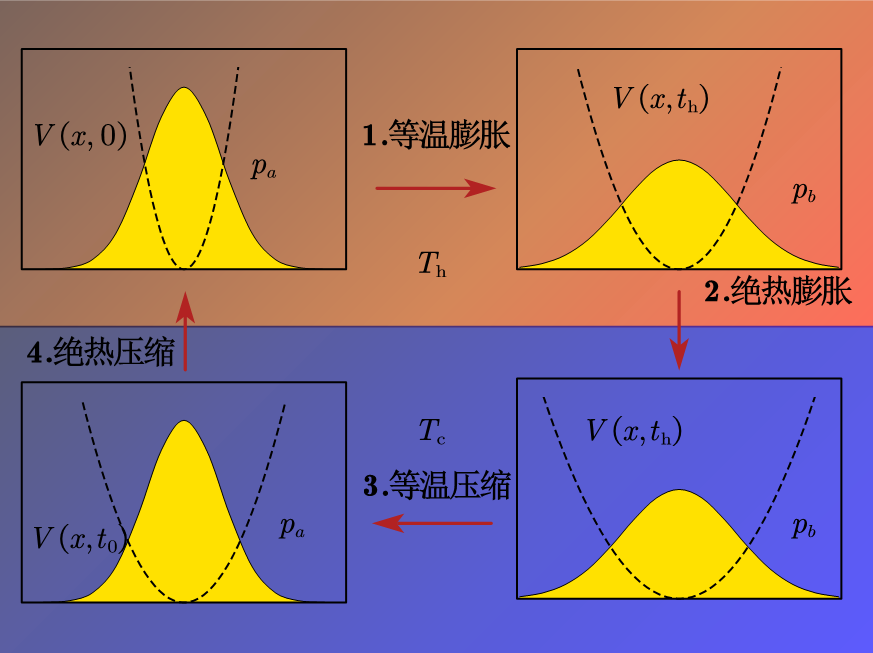
\includegraphics[width=0.5\textwidth]{p2.png}
    \caption{内可逆热机模型}
    \label{f2.07}
\end{figure}

根据这些假设,再联系到轨道功和热量的定义,就能得到一个循环过程的平均功输出
\begin{equation}
    \begin{split}
        -W=\left(T_{\mathrm{h}}-T_{\mathrm{c}}\right) \Delta S-\left({1}/{t_{\mathrm{h}}}+{1}/{t_{\mathrm{c}}}\right) A_{\mathrm{irr}}
    \end{split} 
    \label{eq21.7}
\end{equation}
$A_{\mathrm{irr}}$是不可逆作用量,他们分别除以驱动时间$t_{\mathrm{h}}\text{和}t_{\mathrm{c}}$就得到了相应的不可逆功。而等温膨胀过程中,粒子从高温热源吸收的热量为
\begin{equation}
    \begin{split}
        Q =T_{\mathrm{h}} \Delta S-{A_{\mathrm{irr}}}/{t_{\mathrm{h}}}
    \end{split}
    \label{eq21.8}
\end{equation}
于是可以得到微观随机热机的效率为
\begin{equation}
    \eta \equiv \frac{-W}{Q}=\frac{\left(T_{\M{h}}-T_{\M{c}}\right) \Delta S-\left(\frac{1}{t_{1}}+\frac{1}{t_{3}}\right) A_\M{i r r}}{T_{\M{h}} \Delta S-\frac{A_\M{i r r}}{t_{1}}}
    \label{eq21.9}
\end{equation}
将随机热机的功率$P=-W/(t_{\mathrm{h}}+t_{\mathrm{c}})$,通过优化$t_{\mathrm{h}},\ t_{\mathrm{c}}$取最大值可得,最大功率时热机的效率为
\begin{equation}
    \eta^{*}=\frac{\eta_{\mathrm{C}}}{2-\eta_{\mathrm{C}} / 2}
    \label{eq21.10}
\end{equation}

\section{绝热捷径}
\qquad 在有限时间热力学中,一个非常重要的议题是如何在有限时间内实现不同平衡态的相互转换。绝热捷径\cite{Chen2010}提供了这样一种可以在有限时间内实现平衡态转化的策略。这个策略由 Demirplak and Rice \cite{Demirplak2003}和 Berry \cite{Berry2009} 独立发展出来。在它提出以后的很长一段时间里,引起了一大批研究者的关注。下面我们回顾一下绝热捷径是怎么实现的。


\subsection{绝热捷径的实现}
\qquad 考虑量子力学中的绝热定理\cite{Griffiths2018}:如果一个系统的哈密顿量$H_0(t)$随时间变化很缓慢,即$\tau_\mathrm{e} \gg \tau_\mathrm{i}$,其中$\tau_\mathrm{e}, \tau_\mathrm{i}$分别表示环境的特征时间和系统的内部特征时间。那么如果系统在时间$t=0$处于$H_0 (0)$的本征态,即系统的初态$| \psi(0) \rangle = | n(0) \rangle$,绝热定理告诉我们系统在$t$时刻会处于$H_0 (t)$的对应于瞬时本征态$| n(0) \rangle$,并且
\begin{equation}
    |\psi(t)\rangle=|n(t)\rangle e^{i \theta_{n}(t)} e^{i \gamma_{n}(t)}
    \label{eq2.1}
\end{equation}
其中$\theta_{n}(t)=-\frac{1}{\hbar} \int_{0}^{t} E_{n}(t^{\prime}) \M{d} t^{\prime}, \gamma_{n}(t)=i \int_{0}^{t}\langle n(t^{\prime}) | \partial_{t^{\prime}}n(t^{\prime})\rangle \M{d} t^{\prime}$。注意到,绝热定理实现了$H_0(t)$的对应的本征态之间的转化$| n(0) \rangle \to | n(t) \rangle$。

现在我们考虑取消$\tau_\mathrm{e} \gg \tau_\mathrm{i}$的要求。假设存在一个哈密顿量$H(t)$,它使得系统的态的演化严格为$|\psi(t)\rangle=|n(t)\rangle e^{i \theta_{n}(t)} e^{i \gamma_{n}(t)}$,则根据薛定谔方程有
\begin{equation}
    i \hbar \PP{}{t} |\psi(t)\rangle= H(t) |\psi(t)\rangle
    \label{eq2.2}
\end{equation}
将\eqref{eq2.1}代入\eqref{eq2.2},整理得$ E_{n}+ i \hbar \left( | \partial_{t} n \rangle -\langle n | \partial_t n \rangle\right)|n\rangle=H| n\rangle$,于是可得
\begin{equation}
    \begin{split}
        H(t)&=H_{0}(t)+i \hbar \sum_{m}\left(\left|\partial_{t} m\right\rangle\left\langle m\left|-\left\langle m \mid \partial_{t} m\right\rangle\right| m\right\rangle\langle m|\right) \\
        &\equiv H_0 + H_1
    \end{split}
    \label{eq2.3}
\end{equation}
一个以$H (t)$作为哈密顿量的系统,若其初态为$H_0 (t)$的本征态$| n(0) \rangle$,那么不论$H (t)$随时间的变化快慢与否,在$t$时刻,系统的状态依然是$H_0 (t)$的本征态,只是两者有一个相位差。于是我们实现了在有限时间内的本征态之间的转化。这其中的关键在于我们引进了一个反绝热哈密顿量$H_1 (t)$,根据\eqref{eq2.3},我们已经在形式上得到了$H_1 (t)$。现在我们考虑对于具体的$H_0 (t)$,如何得到$H_1 (t)$的具体表达式。\cite{Jarzynski2013}

让$H_0$通过一系列参数$\bm{\lambda}(t)=\left( \lambda_1 (t) , \lambda_1 (t) , \lambda_1 (t) , \cdot , \lambda_{N} (t) \right)$依赖于时间$t$。同时,$H_0 (\bm{\lambda})$的本征值、本征态为$E_n (\bm{\lambda}),\ | n (\bm{\lambda}) \rangle$,根据复合函数的微分法则,式\eqref{eq2.4}可以写为
\begin{equation}
    H_1 (t)=\dot{\boldsymbol{\lambda}} \cdot \boldsymbol{\xi}(\boldsymbol{\lambda}(t))
    \label{eq2.5}
\end{equation}
其中
\begin{equation}
    \boldsymbol{\xi}(\boldsymbol{\lambda})=i \hbar \sum_{m}(|\boldsymbol{\nabla} m\rangle\langle m|-\langle m \mid \boldsymbol{\nabla} m\rangle| m\rangle\langle m|)
    \label{eq2.4}
\end{equation}
同时$|\nabla m\rangle \equiv \partial_{\boldsymbol{\lambda}}|m(\boldsymbol{\lambda})\rangle,\ \dot{\boldsymbol{\lambda}} \equiv \mathrm{d} \lambda / \mathrm{d} t$

把$\boldsymbol{\xi}$看做参数空间的无穷小平移$\boldsymbol{\lambda} \to \boldsymbol{\lambda} + \delta \boldsymbol{\lambda}$的生成元。这个无穷小平移与希尔伯特空间中态的变换$|\psi\rangle \rightarrow|\psi\rangle+|\delta \psi\rangle$通过以下方式相联系
\begin{equation}
    i \hbar|\delta \psi\rangle=\delta \boldsymbol{\lambda} \cdot \boldsymbol{\xi}|\psi\rangle
    \label{eq2.6}
\end{equation}
这样,在一阶近似下,$H_0 (\bm{\lambda})$的本征态$|n(\bm{\lambda})\rangle$的变换为
\begin{equation}
    |n(\boldsymbol{\lambda})\rangle \rightarrow\left(1+\frac{1}{i \hbar} \delta \boldsymbol{\lambda} \cdot \hat{\boldsymbol{\xi}}\right)|n(\boldsymbol{\lambda})\rangle=e^{i \delta \boldsymbol{\lambda} \cdot \boldsymbol{A}_{n}}|n(\boldsymbol{\lambda}+\delta \boldsymbol{\lambda})\rangle
    \label{eq2.7}
\end{equation}
其中$\boldsymbol{A}_{n}(\boldsymbol{\lambda})=i\langle n | \boldsymbol{\nabla} n\rangle.$ 这意味着,沿着参数空间的曲线$\bm{\lambda}$利用式\eqref{eq2.7},可以将系统的态逐步从$|n(\M{\lambda_0})\rangle$变换成$\M{e}^{i \int_{\bm{\lambda_0}}^{\bm{\lambda_s}}   i\langle n | \boldsymbol{\nabla} n\rangle \M{d}\bm{\lambda}}\left|n\left(\boldsymbol{\lambda}_{s}\right)\right\rangle.$ 这正是们所希望得到的形式。

现在看看系统态的时间演化,先考虑系统经过一个无穷小时间$\delta t$,则态$|\psi \rangle$将演化为
\begin{equation}
     \left(1+\frac{1}{i \hbar} H \delta t\right)|\psi\rangle=|\psi\rangle+\frac{1}{i \hbar} \delta t H_{0}|\psi\rangle+\frac{1}{i \hbar} \delta \boldsymbol{\lambda} \cdot \boldsymbol{\xi}|\psi\rangle
   \label{eq2.8}
\end{equation}
如果考虑态$|\psi \rangle = |n(\bm{\lambda}) \rangle$,那么\eqref{eq2.8}的物理意义就很显然了——$H_0$产生了我们熟悉的动力学相位,而$\boldsymbol{\xi}$产生了几何相因子。

由\eqref{eq2.4}定义的$\bm{\xi}$,也可由下式\eqref{eq2.9}定义(二者的等价性可由$\langle m \mid \boldsymbol{\nabla} n\rangle=\left\langle m\left|\boldsymbol{\nabla} \hat{H}_{0}\right| n\right\rangle /\left(E_{n}-E_{m}\right)$\cite{Berry2009}加以证明)
\begin{subequations}
    \begin{align}
        \left[ \boldsymbol{\xi}, H_{0} \right] &= i \hbar \left( \boldsymbol{\nabla} H_{0}-\operatorname{diag} \left(\boldsymbol{\nabla} H_{0} \right) \right) \label{eq2.9a}\\
        \langle n|\boldsymbol{\xi}| n\rangle &= 0 \label{eq2.9b}
    \end{align}
    \label{eq2.9}
\end{subequations}
其中$\operatorname{diag}\left(\boldsymbol{\nabla} H_{0}\right)=\sum_{m}|m\rangle\left\langle m\left|\boldsymbol{\nabla} H_{0}\right| m\right\rangle\langle m|.$ 对\eqref{eq2.9a}两端同时进行操作$\langle m|\cdots| n\rangle$,得到$\langle m| \boldsymbol{\xi} | n\rangle (E_n - E_m) = \langle m|i \hbar \left( \boldsymbol{\nabla} H_{0}-\operatorname{diag} \left(\boldsymbol{\nabla} H_{0} \right) \right)| n\rangle$. 可见,\eqref{eq2.9a}决定了$\boldsymbol{\xi}$的非对角元,\eqref{eq2.9b}决定了其非对角元。

式\eqref{eq2.9}提供了一种在经典力学中找到反绝热哈密顿量的对应方法。因为我可以利用量子与经典的对应$[A, B]/i \hbar \to \{A, B\}  $将\eqref{eq2.9}转换为经典的,进而可以在经典力学中找到对应的反绝热哈密顿量。现在考虑一个经典系统,其自由度为1,哈密顿量为$H_0 (\bm{\eta};\bm{\lambda}).$ 其中$\bm{\lambda}$依然为依赖于时间的一系列参数,$\bm{\eta}=(q,p)$为广义坐标和广义动量,确定了相空间的一个点。确定的能量$E = H_0 (\bm{\eta};\bm{\lambda})$,将相点约束在相空间的一个能壳上,积分
\begin{equation}
    I(E, \boldsymbol{\lambda}) \equiv \int \mathrm{d} \bm{\eta} \theta\left[E-H_{0}(z ; \boldsymbol{\lambda})\right]
  \label{eq2.10}
\end{equation}
表示的是能壳所围成的体积,阶跃函数$\theta\left[E-H_{0}(z ; \boldsymbol{\lambda})\right]$的存在可以使得积分区域为整个相空间。经典的绝热定理告诉我们$I(E, \boldsymbol{\lambda})$是一个\textbf{绝热不变量} \cite{LiuChuan2019},也就是说如果$H_0$随时间$t$变化得足够缓慢,那么能壳所围成的体积将保持不变。定义任意可观测量$A$的微正则分布平均
\begin{equation}
    \langle A \rangle_{E, \lambda} \equiv \frac{1}{\partial_{E} I} \int \mathrm{d} \bm{\eta} \delta\left(E-H_{0}\right) A
  \label{eq2.11}
\end{equation}
利用函数$I (E,\bm{\lambda})$去定义函数$E (I, \bm{\lambda})$,则有
\begin{equation}
    \boldsymbol{\nabla} E(I, \boldsymbol{\lambda})=-\frac{\boldsymbol{\nabla} I(E, \boldsymbol{\lambda})}{\partial_{E} I(E, \boldsymbol{\lambda})}=\left\langle\boldsymbol{\nabla} H_{0}\right\rangle_{E, \boldsymbol{\lambda}}
  \label{eq2.12}
\end{equation}
其中第一个等式利用了函数的偏导数的性质,第二个等式利用了式\eqref{eq2.10}和式\eqref{eq2.11}。

式\eqref{eq2.9}的经典对应为\cite{Jarzynski1995}
\begin{subequations}
    \begin{align}
        \left\{\boldsymbol{\xi}, H_{0}\right\} &=\boldsymbol{\nabla} H_{0}-\left\langle\boldsymbol{\nabla} H_{0}\right\rangle_{E, \boldsymbol{\lambda}} \equiv \boldsymbol{\nabla} \tilde{H}_{0}    \label{eq2.13a}\\
        \langle\boldsymbol{\xi}\rangle_{E, \boldsymbol{\lambda}} &=0 \label{eq2.13b}
    \end{align}
    \label{eq2.13}
\end{subequations}
其中$\{ \cdots \}$是经典力学中的泊松括号$\{A, B\}=(\partial A / \partial q)(\partial B / \partial p)-(\partial A / \partial p)(\partial B / \partial q)$。利用式\eqref{eq2.12}和泊松括号的定义,式\eqref{eq2.13a}可改写为
\begin{equation}
    \{\boldsymbol{\xi}, i\}=\boldsymbol{\nabla} i
  \label{eq2.14}
\end{equation}
其中关于$\bm{\eta}$和$\bm{\lambda}$的函数$i$的定义为:$i (\bm{\eta}; \bm{\lambda}) \equiv I \left( H_0\left( \bm{\eta}; \bm{\lambda}\right) ; \bm{\lambda} \right)$。类似于量子的情形的,将$\boldsymbol{\xi} (\bm{\eta}; \bm{\lambda})$看做和参数空间的无穷小平移$\boldsymbol{\lambda} \to \boldsymbol{\lambda} + \delta \boldsymbol{\lambda}$相联系的相空间的平移$\bm{\eta} \to \bm{\eta} + \delta \bm{\eta}$的生成元,有\cite{H.1986}
\begin{equation}
    \delta \bm{\eta}=\delta \boldsymbol{\lambda} \cdot\{\bm{\eta}, \boldsymbol{\xi}\}
  \label{eq2.15}
\end{equation}
于是,由式\eqref{eq2.14}和\eqref{eq2.15}可得
\begin{equation}
    \begin{split}
        &i(\bm{\eta}+\delta \bm{\eta} ; \boldsymbol{\lambda}+\delta \boldsymbol{\lambda})-i(\bm{\eta} ; \boldsymbol{\lambda}) \\
        =&\frac{\partial i}{\partial \bm{\eta}} \delta \bm{\eta}+\boldsymbol{\nabla} i \cdot \delta \boldsymbol{\lambda} \\
        =&(\{i, \boldsymbol{\xi}\}+\nabla i) \cdot \delta \boldsymbol{\lambda}\\
        =&0
    \end{split}
    \label{eq2.16}
\end{equation}
这说明,变换$\bm{\eta} \to \bm{\eta} + \delta  \bm{\lambda} \cdot \{\bm{\eta}, \boldsymbol{\xi}\}$将能壳$H_{0}(\bm{\eta} ; \boldsymbol{\lambda})$上的一个相点映射到能壳$H_{0}(\bm{\eta} + \delta \bm{\eta} ; \boldsymbol{\lambda})$上的一个点,而二者包围着相同的相体积。

可见,类似于量子中的情形,只要给经典的系统施加一个反绝热的哈密顿量$\dot{\boldsymbol{\lambda}} \cdot \boldsymbol{\xi}(\bm{\eta}, \boldsymbol{\lambda}(t))$。那么此系统的$I(E, \boldsymbol{\lambda}) \equiv \int \mathrm{d} \bm{\eta} \theta\left[E-H_{0}(z ; \boldsymbol{\lambda})\right]$将严格保持不变,不论$H_0 $随时间的变化快慢与否。这个新的哈密顿量为
\begin{equation}
    H(\bm{\eta}, t)=H_{0}(\bm{\eta} ; \boldsymbol{\lambda}(t))+\dot{\boldsymbol{\lambda}} \cdot \boldsymbol{\xi}(\bm{\eta}, \boldsymbol{\lambda}(t))
    \label{eq2.17}
\end{equation}

\subsection{经典和量子情形下偶次幂势场中生成元的构造}
\label{sec2.3.2}

\qquad 现在,鉴于变换$\bm{\eta} \to \bm{\eta} + \delta  \bm{\lambda} \cdot \{\bm{\eta}, \boldsymbol{\xi}\}$将能壳$H_{0}(\bm{\eta} ; \boldsymbol{\lambda})$ 上的相点映射到了能壳 $ H_{0}(\bm{\eta} + \delta \bm{\eta} ; \boldsymbol{\lambda})$上,我们可以此为根据构造经典力学中的$\boldsymbol{\xi}(\bm{\eta}, \boldsymbol{\lambda})$,下面我们用例子进行说明

考虑一个一维的粒子,处在两堵刚性墙之间,刚性墙的位置为$q=0,\ \lambda$,这个例子这对应于量子力学中的一维无限深势阱。其相空间的能壳如图\eqref{p2.1}所示。
\begin{figure}[!htbp]
    \begin{center}
        \includegraphics[width=0.5\textwidth]{figures/p2.1.pdf}
    \end{center}
    \caption{在一维盒子中的粒子的能壳}
    \label{p2.1}
\end{figure}
系统的哈密顿量为
\begin{equation}
     H_{0}(\bm{\eta} ; \lambda)=\frac{p^{2}}{2}+V_{\mathrm{box}}(q ; \lambda)
        \label{eq2.18}
\end{equation}
其中$V_{\mathrm{box}}(q ; \lambda)$代表一维盒子的势场$V_{\mathrm{box}}(q ; \lambda) = \left\{\begin{array}{l} 0 ,\ q<\lambda\\ \infty ,\ q \leq 0\ \text{or}\ q \geq \lambda \end{array}\right.$在经典中这个粒子的运动是平凡的——以相同的速度在两堵墙之间做往返运动。
    
哈密顿量的参数$\lambda$随时间$t$变化,现在我们构造这个系统的反绝热哈密顿量。不难得出,矩形能壳的面积为$I=2 \bar{p} \lambda$,由于矩形能壳的长的变化为$\lambda \to \lambda(1+\nu)$,为了维持矩形能壳的面积,在一阶精度下,可令其宽的微小改变为$2 \bar{p} \to 2 \bar{p} (1-\nu)$,其中$\nu \equiv \delta \lambda / \lambda$。于是,这两个能壳被一个线性的尺度变换所联系
\begin{equation}
    q \rightarrow q(1+\nu) \quad, \quad p \rightarrow p(1-\nu)
    \label{eq2.19}
\end{equation}
现在我们可以通过$(\nu q, -\nu p)  = \delta \lambda \{ (q, p), \xi \}$(式\eqref{eq2.15})逆向解出生成元的表达式,于是我们可得一对这样的方程$\left\{ \begin{array}{l} q / \lambda=\partial \xi / \partial p \\ p / \lambda=\partial \xi / \partial q \end{array}\right.$。结合限制条件\eqref{eq2.13b},于是可令$\xi = q p / \lambda$。再根据式\eqref{eq2.19},我们最终得到
\begin{equation}
    H(\bm{\eta}, t)=H_{0}(\bm{\eta} ; \lambda)+\frac{\dot{\lambda}}{\lambda} q p \quad, \quad \lambda=\lambda(t)
    \label{eq2.20}
\end{equation}
在这个时间依赖的哈密顿量之下,绝热不变量$i(q, p;\ \lambda)=2 |p| \lambda$是严格守恒的,不论函数$\lambda(t)$的形式是怎样的。现在我们对于这个具体的例子,实实在在的构造出了反绝热哈密顿量,这说明其并不只是存在于形式化理论中,而是可以在实际中加以利用的。

在构造出了经典的反绝热哈密顿量之后,我们也可以通过$\xi$的经典表达式来猜想量子力学中的反绝热哈密顿量,因为算符$p, q$是不对易的,一个自然的猜想是
\begin{equation}
    \xi(\lambda) = \frac{q p + p q}{2 \lambda}
    \label{eq2.21}
\end{equation}
于是,再联系到已知的量子力学中一维无限深势阱的本征解,非常幸运地,我们发现选择的这个$\xi$满足式\eqref{eq2.7}
\begin{equation}
    \left(1+\frac{1}{i \hbar} \delta \lambda \xi \right) \sqrt{\frac{2}{\lambda}} \sin \left(\frac{n \pi q}{\lambda}\right)=\sqrt{\frac{2}{\lambda+\delta \lambda}} \sin \left(\frac{n \pi q}{\lambda+\delta \lambda}\right)
    \label{eq2.22}
\end{equation}
这一点可以通过计算$\PP{}{\lambda} \sqrt{\frac{2}{\lambda}} \sin \left(\frac{n \pi q}{\lambda}\right) \delta \lambda = \frac{1}{i \hbar} \delta \lambda \xi \sqrt{\frac{2}{\lambda}} \sin \left(\frac{n \pi q}{\lambda}\right)$得到验证。\eqref{eq2.22}中的相位由于$A_{n}(\lambda)=i\langle n | \partial_\lambda  n\rangle = 0$而消失。于是可以立刻得到
\begin{equation}
    H(t)=-\frac{\hbar^{2}}{2 m} \frac{\partial^{2}}{\partial q^{2}}+V_{\mathrm{box}}(q ; \lambda)+\frac{\dot{\lambda}}{2 \lambda} \frac{\hbar}{i}\left(q \frac{\partial}{\partial q}+\frac{\partial}{\partial q} q\right)
    \label{eq2.23}
\end{equation}
这样,波函数
\begin{equation}
    \psi (q, t)=\sqrt{\frac{2}{\lambda}} \sin \left(\frac{n \pi q}{\lambda}\right) \exp \left(-\frac{i}{\hbar} \int_{0}^{t} \mathrm{~d} t^{\prime} \frac{n^{2} \pi^{2} \hbar^{2}}{2 m \lambda^{2}}\right)
    \label{eq2.24}
\end{equation}
将成为这个系统的精确解(初态为$\psi (q, 0) = \sqrt{\frac{2}{\lambda}} \sin \left(\frac{n \pi q}{\lambda}\right)$),不论$\lambda(t)$的函数形式如何。式\eqref{eq2.23}也可以更一般的写成
\begin{equation}
    \left(1+\frac{1}{i \hbar} \delta \lambda \hat{\xi}\right) \psi(q)=\sqrt{\frac{1}{s}} \psi\left(\frac{q}{s}\right) \quad, \quad s=\frac{\lambda+\delta \lambda}{\lambda}
    \label{eq2.25}
\end{equation}
换句话说,算符$\exp (\delta \lambda \xi / i \hbar)$对波函数$\psi(q)$进行了线性放大。(系数$\sqrt{\frac{1}{s}}$保证了波函数的归一化)自此我们也成功的通过构造的经典反绝热哈密顿量构造出了量子反绝热哈密顿量

不难发现,我们的构造能够成功,很大程度上得益于能壳和本征态之间的尺度变换关系能够成立。相似的办法也能够应用于偶次幂势场,则经典哈密顿量为
\begin{equation}
    H_{0}(\bm{\eta} ; \lambda)=\frac{p^{2}}{2 m}+\epsilon\left(\frac{q}{\lambda}\right)^{b}
    \label{eq2.26}
\end{equation}
可以证明,对于相应的量子的情形,也是可以按照类似的方式构造其量子反绝热哈密顿量的。其中$\epsilon > 0$调节了能量尺度,而$b$是正偶数。同样的,我们先在经典中加以考虑,再推广到量子中。上述系统的绝热不变量为
\begin{equation}
    \begin{split}
        i(\bm{\eta};\ \lambda) &= 4 \int_0^{\lambda \left(H_0 / \epsilon \right)^{1/b}} \sqrt{2 m \left[ H_0 -\epsilon \left(q/{\lambda}\right)^b\right]} \, \M{d}q \\ 
        &= \sqrt{8 \pi m} \epsilon^{-1 / b} \frac{\Gamma\left(1+\frac{1}{b}\right)}{\Gamma\left(\frac{3}{2}+\frac{1}{b}\right)} \lambda H_0^{\frac{1}{2 \mu}}\\
        &= c \lambda H_0^{\frac{1}{2 \mu}}
    \end{split}
    \label{eq2.27}
\end{equation}
其中,$\mu \equiv \frac{b}{b+2} , c \equiv \sqrt{8 \pi m} \epsilon^{-1 / b} \frac{\Gamma\left(1+\frac{1}{b}\right)}{\Gamma\left(\frac{3}{2}+\frac{1}{b}\right)}$
同样的,含时参数$\lambda \to \lambda + \delta \lambda$的变化,通过一个线性变换引起了能壳的变化。为了看到这一点,我们考虑$i(q, p;\ \lambda)$的变化$\delta i(q, p;\ \lambda) = \PP{i}{q} \delta q + \PP{i}{p} \delta p + \PP{i}{\lambda} \delta \lambda \equiv 0$,为了使恒等式成立,可以假设$\delta q = x q \frac{\delta \lambda}{\lambda}, \delta p = - y p \frac{\delta \lambda}{\lambda}$,可以得到
\begin{equation}
    \frac{c}{2 \mu H_0} \left[ (\mu - y) \frac{p^2}{m} + (2 \mu - b + b x) \epsilon \left( \frac{q}{\lambda} \right)^b \right] \delta \lambda \equiv 0
    \label{eq2.28}
\end{equation}
要使上式成立,必须有$x=y=\mu$,可见,能壳的变换依然可以由式\eqref{eq2.19}进行描述,只不过现在$\nu = \mu \delta \lambda / \lambda$,同理我们可以得到新的哈密顿量
\begin{equation}
    H(\bm{\eta}, t)=H_{0}(\bm{\eta} ; \lambda)+\mu \frac{\dot{\lambda}}{\lambda} q p
    \label{eq2.28.5}
\end{equation}
在这个哈密顿量下,$i(\bm{\eta};\ \lambda) = c \lambda H_0^{\frac{1}{2 \mu}}$将成为一个严格的守恒量。在量子力学中,势场\eqref{eq2.26}的本征态将满足
\begin{equation}
    \phi_{n}(q ; \lambda)=\sqrt{\frac{1}{\lambda^{\mu}}} \phi_{n}\left(\frac{q}{\lambda^{\mu}} ; 1\right)
    \label{eq2.29}
\end{equation}
新的哈密顿量为
\begin{equation}
    H(t)=H_{0}(\lambda)+\frac{b}{b+2} \frac{\dot{\lambda}}{2 \lambda} \frac{\hbar}{i}\left(q \frac{\partial}{\partial q}+\frac{\partial}{\partial q} q\right)
    \label{eq2.29.5}
\end{equation}
之下。这个结果对任意$b \in \{ 2, 4, 6, \cdots\}$都是成立的。特别地,$b=2$和$b \to \infty$对应于一维谐振子和一维无限深势阱的情况。不过,对于一维谐振子的情况,Muga等人使用升降算子$a, a^{\dagger}$结合式\eqref{eq2.3}的办法更为简单地得到了相同的结果。\cite{Muga2010}

对于一般的一维势场,生成元应该满足
\begin{equation}
    \boldsymbol{\xi}\left(\bm{\eta}_{b} ; \boldsymbol{\lambda}\right)-\boldsymbol{\xi}\left(\bm{\eta}_{a} ; \boldsymbol{\lambda}\right)=\int_{a}^{b} \mathrm{~d} t \nabla \tilde{H}_{0}(\bm{\eta}(t) ; \boldsymbol{\lambda})
    \label{eq2.30}
\end{equation}
其中相点$\bm{\eta}_{a}, \bm{\eta}_{b}$在同一能壳上,$\bm{\eta}(t)$是相点从$\bm{\eta}_{a}$演化到$\bm{\eta}_{b}$的相轨迹。式\eqref{eq2.30}可以结合式\eqref{eq2.13a}和$(\mathrm{d} / \mathrm{d} t) \boldsymbol{\xi}(\bm{\eta}(t) ; \boldsymbol{\lambda})=\left\{\boldsymbol{\xi}, H_{0}\right\}$而得到。

如果我们考虑相空间中复杂一点的能壳,它们不是简单闭合的环。比如如果势$V(q;\ \bm{\lambda})$是双阱势,而参数$\bm{\lambda}$的变化可以改变能壳的拓扑结构——从单环变成双环或相反。这时$i$的绝热不变性将被破坏。\cite{Tennyson1986,Cary1986,Hannay1986}

对于自由度$f \geq 2$的经典系统,如果$H_0$是完全可积的\cite{LiuChuan2019},我们就有可能能够重复
式\eqref{eq2.10}-\eqref{eq2.17}对作用量-角度变量的分析,每一个生成元$\bm{\xi}_i$对应一对作用量-角度变量。另外,如果$H_0$是各态历经的,那么式$\eqref{eq2.13a}$的解的存在将意味着能壳$H_0 (\bm{\eta};\ \bm{\lambda})$可以被正则变换到$H_0 (\bm{\eta};\ \bm{\lambda}+\delta \bm{\lambda} )$。\cite{Jarzynski1995}虽然对于$f \geq 2$的系统,这一条件通常并不能被满足,但一旦满足,$\bm{\xi}$就简单的是这个变换的生成元。

\subsection{利用绝热捷径实现平衡态的转化}
\qquad 接下来我们举例说明绝热捷径如何实现平衡态的转化。\cite{Tu2013}考虑一个被依赖于时间的谐振子势场$U_0 (q, \lambda(t))= q^{2} / 2 \lambda(t)^2$驱动的布朗粒子,只需使式\eqref{eq2.26}中的$b=2,\ \epsilon=2$,再联系到式\eqref{eq2.29},就可以直接得到它被施加反绝热哈密顿量之后的哈密顿量
\begin{equation}
    \begin{split}
    H(t)=&H_0 (t) + \frac{\dot{\lambda}}{2 \lambda(t)} q p\\
    =&\frac{p^{2}}{2}+\frac{1}{2}\frac{q^2}{\lambda(t)^2}+\frac{\dot{\lambda}}{2 \lambda(t)} q p
    \end{split}
    \label{eq2.31}
\end{equation}
在时间$t_i < t \leq t_f$内,参数由$\lambda_{i} \equiv \lambda(t_i)$变为$\lambda_{f} \equiv \lambda(t_f)$。我们要求
\begin{equation}
    \dot{\lambda}\left(t_{i}\right)=\dot{\lambda}\left(t_{f}\right)=0,
    \label{eq2.31.5}
\end{equation}
这样才有$H\left(t_{f}\right)=H_0 \left(t_{f}\right), H\left(t_{f}\right)=H_0 \left(t_{f}\right)$,除此之外,$\lambda (t)$依赖于时间$t$的形式有很大的任意性。运动方程为
\begin{equation}
    \left\{\begin{aligned}
        &\dot{q}=\frac{\partial H}{\partial p}={p}+\frac{\dot{\lambda}}{2 \lambda(t)} q \\
        &\dot{p}=-\frac{\partial H}{\partial q}=-\frac{q}{\lambda^{2}(t)}-\frac{\dot{\lambda}(t)}{2 \lambda(t)} p
        \end{aligned}\right.
    \label{eq2.31.7}
\end{equation}


接下来我们将说明绝热捷径如何联系两个不同有效温度的正则态。\cite{Tu2013}假设系统初始处在有效温度为$\left(k_\M{B} \beta_i\right)^{-1}$的正则态中,那么初始时系统的分布函数可以表达为
\begin{equation}
    \rho_{i}=\frac{\beta_{i}}{2 \pi \lambda_{i}} \exp \left[-\beta_{i} H_0 \left(t_{i}\right)\right]
    \label{eq2.32}
\end{equation}
其中$(q_i, p_i)$代表初始时的相点,根据刘维尔定理,当系统不和外界任何热浴接触时,分布函数沿着相轨应当是不变的。所以,末态的分布函数应当为
\begin{equation}
    \rho_{f}=\rho_{i}=\frac{\beta_{i} }{2 \pi \lambda_{i}} \exp \left[-\beta_{i} H_0 \left(t_{i}\right)\right]
    \label{eq2.33}
\end{equation}
接着我们寻找末态的有效温度,使得末态的分布函数\eqref{eq2.33}可以被表达成正则分布的样子
\begin{equation}
    \rho_{f}=\frac{\beta_{f} }{2 \pi \lambda_{f}} \exp \left[-\beta_{f} H_0 \left(t_{f}\right)\right]
    \label{eq2.34}
\end{equation}
其中$(q_f, p_f)$是末态的相点。计算$H_0 (t)$对时间的导数得
\begin{equation}
    \begin{split}
        \DD{H_0 (t)}{t} =& \frac{p}{m}\dot{p} + 2 \epsilon \frac{q}{\lambda^2}\dot{q} - \frac{q^2}{\lambda^2} \dot{\lambda}\\
                        =& -H_0 (t) \DD{\ln{\lambda(t)}}{t}
    \end{split}
    \label{eq2.35}
\end{equation}
第二个等式用到了运动方程\eqref{eq2.34}于是可得$H_0 \left(t_{f}\right)=H_0 \left(t_{i}\right) \lambda_{i} / \lambda_{f}$,将这个式子代入式\eqref{eq2.34},得到
\begin{equation}
    \rho_{f}=\frac{\beta_{f} }{2 \pi \lambda_{f}} \exp \left[-\frac{\beta_{f} \lambda_i}{\lambda_f} H_0 \left(t_{f}\right)\right]
    \label{eq2.36}
\end{equation}
将这个式子和式\eqref{eq2.33}比较可得
\begin{equation}
    \frac{\beta_f}{\lambda_f} = \frac{\beta_i}{\lambda_i}
    \label{eq2.40}
\end{equation}
这说明,如果系统的初态等效温度为$\beta_{i}^{-1}$的正则态,那么在系统经历绝热捷径之后,我们可以把系统的末态视为等效温度为$\beta_{f}^{-1}$的正则态。而且,初态和末态的等效温度满足\eqref{eq2.40}。

这样,通过绝热捷径,在有限时间时间$t_i \sim t_f$内,我们实现了微观正则态之间的转换。


\section{等温捷径}
    
\qquad 上一节我们介绍了绝热捷径,它可以在有限时间内实现两个不同有效温度的正则平衡态之间的转化。又由于这个过程中,系统和外界没有热交换故而称之为绝热捷径。那么类比于经典中的绝热过程和等温过程,我自然难免思考是否会存在对应的等温捷径。类似的,我们希望它可以在有限时间内实现两个等温平衡态间的转化。

Martínez\cite{Martinez2016}针对谐振子场中的布朗粒子,通过对劲度系数进行调节,使系统比自然驰豫过程快一百倍达到了平衡态。Le Cunuder等人\cite{LeCunuder2016}实现了微观谐振子平衡态的快速转化。不过这些方法都只能限制于布朗粒子系统,我们需要在一般情况也能适用的办法。于是,李耿等人\cite{Li2016}发展出了等温捷径的概念。很类似于绝热捷径,李耿等人为一个初始处于平衡态的系统施加了一个辅助势场(类似于绝热捷径中的反绝热哈密顿量),它使得这个和恒温热浴接触的系统的演化处于原哈密顿量的瞬时平衡态。通过对辅助势场的调节,可以使得系统的初末状态都是原哈密顿量的平衡态,就此实现了等温情况下平衡态间的转化。

\subsection{等温捷径的实现}


\qquad 考虑一个和温度为$T$的热浴接触的系统,如果系统的哈密顿量$H_0 \left(\bm{\eta}, \lambda\left( t \right) \right)$依赖于时间。分布函数$\rho (\bm{\eta}, t)$的时间演化由下式决定
\begin{equation}
    \frac{\partial \rho(\bm{\eta}, t)}{\partial t}=L_{0}(\bm{\eta}, \lambda(t)) \rho(\bm{\eta}, t)
    \label{eq2.41}
\end{equation}
其中$L_{0}(\bm{\eta}, \lambda(t))$是演化算符,我们将讨论的框架限制在这样一种情况下:对于固定的参数$\lambda$,系统处于这样一种平衡态之中,它的分布函数满足$\rho_{\mathrm{eq}} \propto e^{-\beta H_{0}(\bm{\eta}, \lambda)}$。现在给系统引入一个辅助势$U_1 (\bm{\eta}, t)$,哈密顿量成为$H(\bm{\eta}, t)=H_{0}(\bm{\eta}, \lambda(t))+U_{1}(\bm{\eta}, t)$,演化方程\eqref{eq2.41}成为
\begin{equation}
    \frac{\partial \rho(\bm{\eta}, t)}{\partial t}=L_{0}(\bm{\eta}, \lambda(t)) \rho(\bm{\eta}, t)+L_{1}(\bm{\eta}, t) \rho(\bm{\eta}, t)
    \label{eq2.42}
\end{equation}
其中$L_{1}(\bm{\eta}, t)$代表与辅助势对应的算符。我们要求辅助势可以使得系统在任何时候都处于原哈密段量的瞬时平衡态中,则分布函数为
\begin{equation}
    \rho(\bm{\eta}, t)=\rho_{\mathrm{ieq}}(\bm{\eta}, \lambda(t)) \equiv e^{\beta\left[F(\lambda(t))-H_{0}(\bm{\eta}, \lambda(t))\right]}
    \label{eq2.43}
\end{equation}
其中,$F(\lambda) \equiv-\beta^{-1} \ln \left[\int e^{-\beta H_{0}(\bm{\eta}, \lambda)} \M{d} \bm{\eta}\right]$是原系统在给定参数$\lambda$时,在平衡态下的自由能。\eqref{eq2.43}的积分是对整个相空间的。如果我们限制辅助势$U_1 (\bm{\eta} , t)$在驱动过程的初末时刻都为零,即分布函数在初末时刻都对应于哈密顿量$H(\bm{\eta}\ , t)$,那么我们就实现了有限时间内的等温平衡态的转化。

上面的这种方法看上去很类似于Vaikuntanathan和Jarzynski提出的护送自由能模拟(escorted free-energy simulations)。\cite{Vaikuntanathan2008}通过在系统中引入恰当的人工场流和巧妙的功的定义,这个方法可以生成相轨迹,沿着这些相轨迹做的功等于系统自由能的改变。而等温捷径的方法致力于为等温情况下有限时间内平衡态的转化提供统一的理论框架。也不用额外引入功的定义,可以依旧采用随机热力学中轨道功的定义。\cite{Seifert2012,Sekimoto2010}

\subsection{等温捷径应用于过阻尼布朗粒子}

\qquad 考虑在势场$U_0 (q, \lambda(t))$中的一维布朗粒子,在过阻尼的情形下忽略其惯性的影响。为系统引入一个辅助势$U_1 (q,t)$,那么现在粒子的势场为
\begin{equation}
    U (q,t) = U_0 (q, \lambda(t)) + U_1 (q,t)
    \label{eq2.44}
\end{equation}
布朗粒子的分布函数$\rho (q, t)$的演化由福克-普朗克方程\eqref{eq2.45}决定。鉴于我们的假设——系统时刻处在$H_0 (\bm{\eta}, \lambda(t))$瞬时平衡态下,则系统的分布函数为
\begin{equation}
    \rho(q, t)=\rho_{\mathrm{ieq}}(q, \lambda(t)) \equiv \mathrm{e}^{\beta\left[F(\lambda(t))-U_{0}(q, \lambda(t))\right]}
    \label{eq2.46}
\end{equation}
其中,$F(\lambda) \equiv-\beta^{-1} \ln \left[\int_{-\infty}^{+\infty} e^{-\beta U_{0}(q, \lambda)} \M{d} q \right]$将式\eqref{eq2.46}代入福克-普朗克方程\eqref{eq2.45},可以得到$U_1 (q,t)$需要满足的方程:
\begin{equation}
    \frac{1}{\gamma \beta} \frac{\partial^{2} U_{1}}{\partial q^{2}}-\frac{1}{\gamma} \frac{\partial U_{0}}{\partial q} \frac{\partial U_{1}}{\partial q}=\left(\frac{\M{d} F}{\M{d} \lambda}-\frac{\partial U_{0}}{\partial \lambda}\right) \dot{\lambda}
    \label{eq2.47}
\end{equation}
可以令$ U_{1}(q, t)$取如下形式
\begin{equation}
    U_{1}(q, t)=\dot{\lambda}(t) f(q, \lambda(t))
    \label{eq2.48}
\end{equation}
将上式\eqref{eq2.48}代入式\eqref{eq2.47}可得
\begin{equation}
    \frac{1}{\gamma \beta} \frac{\partial^{2} f}{\partial q^{2}}-\frac{1}{\gamma} \frac{\partial U_{0}}{\partial q} \frac{\partial f}{\partial q}=\frac{d F}{d \lambda}-\frac{\partial U_{0}}{\partial \lambda}
    \label{eq2.49}
\end{equation}
非常有趣的是式\eqref{eq2.46}是方程\eqref{eq2.49}的积分因子,于是不难求得方程\eqref{eq2.49}的形式解。再结合假设\eqref{eq2.48},得到
\begin{equation}
    U_{1}(q, t)=\gamma \beta \dot{\lambda}(t) \int \M{d} q \frac{\int \M{d} q h(q, \lambda(t))}{\rho_{\mathrm{ieq}}(q, \lambda(t))}
    \label{eq2.50}
\end{equation}
其中$h(q, \lambda) \equiv\left[\frac{\M{d} F(\lambda)}{\M{d} \lambda}-\frac{\partial U_{0}(q, \lambda)}{\partial \lambda}\right] \rho_{\mathrm{ieq}}(q, \lambda)$。注意到,从分布函数的演化得到势能的想法,Martínez等人在快速平衡(engineered swift equilibration)的研究\cite{Martinez2016}中已经应用过。不过,我们是从给定的势能$U_0 (q,\lambda(t))$得到辅助势,Martínez等人是从给定的分布函数得到辅助势。而且,Martínez等人的方法不能同时确定哈密顿量和自由能。

考虑到我们对辅助势的$U(q,t)$限制条件——在驱动过程的初末时刻$t_i,\ t_f$要使得$U(q,t)=U_0 (q,t)$,于是我们引入限制条件
\begin{equation}
    \dot{\lambda}(t_i)=\dot{\lambda}(t_f)=0
    \label{eq2.51}
\end{equation}
结合辅助势\eqref{eq2.50}和上式\eqref{eq2.51}的边界条件,我们就在过阻尼的情况下实现了等温捷径。

现在来让我们考虑两个简单的例子,第一个例子是在谐振子中受时间依赖的力的布朗粒子。相应的势能为
\begin{equation}
    U_{0}(q, \lambda(t))=\frac{1}{2} k q^{2}-\lambda(t) q
    \label{eq2.52}
\end{equation}
其中$k$代表了谐振子势的强度,$\lambda(t)$是外力。将上式\eqref{eq2.52}代入式\eqref{eq2.50}就得到了辅助势的形式
\begin{equation}
    U_{1}(q, t)=-\frac{\gamma \dot{\lambda}(t)}{k} q
    \label{eq2.53}
\end{equation}
再来看一个例子:依赖于时间的谐振子势场中的布朗粒子,势场为
\begin{equation}
    U_{0}(q, \lambda(t))=\frac{q^2}{2 \lambda(t)^2}
    \label{eq2.54}
\end{equation}
同样的,根据式\eqref{eq2.50}可得辅助势为
\begin{equation}
    U_{1}(q, t)=-\frac{\gamma \dot{\lambda}(t)}{2 \lambda(t)} q^{2}
    \label{eq2.55}
\end{equation}
式\eqref{eq2.55}和Martínez等人得到的结果\cite{Martinez2016}是等价的。并且,他们的结果意味着对于势场$U_0 (q, \lambda(t))= q^{n} / 2 \lambda(t)^n   \quad (n=2,4,6\cdots)$都可以找到辅助势的解析解$U_{1}(q, t)=- \gamma \dot{\lambda} q^{2} /(2  \lambda)$。除此之外,也可以找到另一类势场$U_{0}(q, \lambda(t))=u(q-\lambda(t))$的辅助势\cite{Li2016},这是一个随时间平移的势场,相应的辅助势为$U_{1}(q, t)=-\gamma \dot{\lambda} q$。


\subsection{等温捷径应用于欠阻尼布朗粒子}
\qquad 在欠阻尼情况下,布朗粒子的惯性的影响不能忽略,我们假设辅助势$U_1$是粒子的坐标$q$和动能$p$的函数\footnote{严格说来,这个时候$U_1 (q,p)$ 应该叫做辅助哈密顿量。}。则总哈密顿量为
\begin{equation}
    H(q, p, t)=H_{0}(q, p, \lambda(t))+U_{1}(q, p, t)
    \label{eq2.56}
\end{equation}
其中$H_{0}(q, p, \lambda(t))=p^{2}/{2}+U_{0}(q, \lambda(t))$。但是通常的福克-普朗克方程\eqref{eq12.57}只能描述势场不依赖于动量$p$时分布函数$\rho (q,p,t)$的时间演化。仿照Reichl对福克-普朗克方程的推导\cite{Reichl2016},李耿得到了势能含有动量$p$的福克-普朗克方程\cite{Li2016},如下
\begin{equation}
        \PP{\rho}{t} + \nabla \cdot \bm{J} = 0
    \label{eq2.57}
\end{equation}
其中
\begin{equation}
    \bm{J} \equiv \rho \left( p + \PP{U}{p} \right) \hat{\mathbf{q}}-\rho\left(\gamma p+\frac{\partial U}{\partial q}+ \PP{U}{p} + \frac{\gamma}{\rho \beta} \frac{\partial \rho}{\partial p}\right) \hat{\mathbf{p}}
\label{eq2.57.5}
\end{equation}
注意到,我们令$U \equiv U_0 + U_1$,算符$\nabla \equiv \hat{\mathbf{q}} \partial / \partial x+\hat{\mathbf{p}} \partial / \partial p$,其中$\hat{\mathbf{q}}$和$\hat{\mathbf{p}}$是单位方向向量。
原系统瞬时平衡态的分布函数为
\begin{equation}
    \rho(q, p, t)=\rho_{\mathrm{ieq}}(q, p, \lambda(t)) \equiv \mathrm{e}^{\beta\left[F(\lambda(t))-H_{0}(x, p, \lambda(t))\right]}
    \label{eq2.58}
\end{equation}
其中$F(\lambda) \equiv-\beta^{-1} \ln \left[\int_{-\infty}^{+\infty} \M{d} q \int_{-\infty}^{+\infty} \M{d} p e^{-\beta H_{0}(q, p, \lambda)}\right]$
同理,将上式\eqref{eq2.58}代入方程\eqref{eq2.57},得到
\begin{equation}
    \frac{\gamma}{\beta} \frac{\partial^{2} U_{1}}{\partial p^{2}}-\gamma p \frac{\partial U_{1}}{\partial p}+\frac{\partial U_{0}}{\partial q} \frac{\partial U_{1}}{\partial p}-p \frac{\partial U_{1}}{\partial q}=\left(\frac{d F}{d \lambda}-\frac{\partial U_{0}}{\partial \lambda}\right) \dot{\lambda}
    \label{eq2.59}
\end{equation}
假设$U_{1}(q, p, t)=\dot{\lambda}(t) f(q, p, \lambda(t))$,可以得到关于$f$的偏微分方程
\begin{equation}
    \frac{\gamma}{\beta} \frac{\partial^{2} f}{\partial p^{2}}-\gamma p \frac{\partial f}{\partial p}+\frac{\partial U_{0}}{\partial q} \frac{\partial f}{\partial p}-p \frac{\partial f}{\partial q}=\frac{d F}{d \lambda}-\frac{\partial U_{0}}{\partial \lambda}
    \label{eq2.60}
\end{equation}
不同于欠阻尼的情况,除了一些特殊情况,我们无法为上面这个方程\eqref{eq2.60}找到解析解。

和欠阻尼的情况一样,依然考虑两个特殊的势场\eqref{eq2.52}和\eqref{eq2.54}。可以求得相应的辅助势为
\begin{equation}
    U_{1}(q, p, t)=\frac{\dot{\lambda}(t)}{k}(p-\gamma q)
    \label{eq2.61}
\end{equation}
和
\begin{equation}
    U_{1}(q, p, t)=-\frac{\dot{\lambda}(t)}{2 \gamma \lambda(t)}\left[(p-\gamma q)^{2}+ q^{2}/\lambda(t)^2\right]
    \label{eq2.62}
\end{equation}
类似于过阻尼的情形,在欠阻尼的情形下我们也可以为两类势场的辅助势找到解析解\cite{Li2016},势场$U_0 (q, \lambda(t))= q^{n} / 2 \lambda(t)^n \quad (n=2,4,6\cdots) ,\ U_{0}(q, \lambda(t))=u(q-\lambda(t))$的辅助势分别为$U_{1}(q, p, t) = - \dot{\lambda}\left[(p-\gamma q)^{2}+ q^{n}/\lambda(t)^n \right] / 2  \gamma \lambda ,\ U_{1}(q, p, t)=\dot{\lambda}(p-\gamma q)$。













\chapter{绝热捷径与等温捷径构成的类卡诺循环热机}
\section{布朗粒子的能量学}
\qquad 在正式开始讨论我们构建的热机之前,为了方便讨论热机的效率、熵变等问题,让我们先花一点时间讨论布朗粒子的能量学。
\subsection{过阻尼布朗粒子的能量学}
\R{李耿博士毕业论文,第一章随机能量学可作为参考}

考虑一个和温度为$T$的热浴接触的一维布朗粒子。它被施加一个依赖于时间的外势$U(q,p,t) = U_0 (q,\lambda(t)) + U_1 (q,t)$,其中考虑到了在绝热捷径和等温捷径中我们施加的辅助势$U_1$。在过阻尼情况下,粒子的惯性的影响可以忽略,哈密顿量为
\begin{equation}
    H=U_0 (q,\lambda(t)) + U_1 (q,p,t)
    \label{eq31.1}
\end{equation}
哈密顿量的全微分为
\begin{equation}
    \M{d} H=\left(\dot{q} \frac{\partial U_0}{\partial q} + \dot{q} \P1P{U_1}{q}  \right) \M{d} t+\left(\dot{\lambda} \frac{\partial U_0}{\partial \lambda} + \P1P{U_1}{t} \right) \M{d} t
    \label{eq31.2}
\end{equation}
这提示我们定义沿着相轨迹$(q(t), p(t))$的能量差\cite{Tu2013}
\begin{equation}
     \Delta e \equiv H\left(t_{f}\right)-H\left(t_{i}\right),
     \label{eq31.3}
\end{equation}
输入功
\begin{equation}
    w \equiv \int_{t_{i}}^{t_{f}} \M{d} t \left( \dot{\lambda} \frac{\partial U_0}{\partial \lambda} + \P1P{U_1}{t} \right)
    \label{eq31.4}
\end{equation}
这也与传统的随机热力学对轨道功的定义相符合。\cite{Sekimoto2010,Jarzynski1997,Sekimoto_1997}。还有吸收的热量
\begin{equation}
    q \equiv \int_{t_{i}}^{t_{f}} \M{d} t \dot{q} \frac{\partial U}{\partial q} .
    \label{eq31.5}
\end{equation}
相轨连接了初时刻$t_i$对应的相点$(q_i , p_i )$和末时刻$t_f$对应的相点$(q_f , p_f )$。显然,对于每条相轨有
\begin{equation}
    \Delta e = w + q
    \label{eq31.6}
\end{equation}

而系统的分布函数$\rho (q,p,t)$由的福克-普朗克-克拉马斯方程\eqref{eq2.45}决定,在知道了$\rho (q,p,t)$之后就可以计算以上式子\eqref{eq31.4}-\eqref{eq31.6}的系综平均,这和文献\cite{Seifert2005,Shizume1995,Bizarro2011}的步骤是类似的。得到能量差和输入功的系综平均为
\begin{equation}
    \Delta E \equiv\langle\Delta e\rangle=\left.\int \M{d} q (H \rho)\right|_{t_{i}} ^{t_{f}} ,
    \label{eq31.7}
\end{equation}
和
\begin{equation}
    W \equiv\langle w\rangle=\int_{t_{i}}^{t_{f}} \M{d} t \int \M{d} q \left[\rho \left( \dot{\lambda} \frac{\partial U_0}{\partial \lambda} + \P1P{U_1}{t} \right) \right].
    \label{eq31.8}
\end{equation}

对于吸收的热的系综平均,由于存在$\dot{q}$,我们不好直接积分,需要做进一步的推导。系综平均为
\begin{equation}
    Q=\int_{t_i}^{t_f}\left\langle\dot{q} \frac{\partial U}{\partial q} \right\rangle \mathrm{d} t
    \label{eq31.9}
\end{equation}
现在分两步对上式\eqref{eq31.9}进行平均。

第一步,对系综中在$t$时刻经过$q$的轨道进行平均\R{(不懂至以下)},得到
\begin{equation}
    \langle\dot{x} \mid x, p, t\rangle=\frac{J}{\rho}
    \label{eq31.10}
\end{equation}
其中$J$是式\eqref{eq2.45.5}所定义的流。

第二步,利用分布函数$\rho(q,p,t)$对所有的$q$和$p$进行系综平均。于是,系统与热浴的热交换为
\begin{equation}
    \begin{split}
        Q&=\int_{t_i}^{t_f} \mathrm{d} t \int \mathrm{d} q \left(J \frac{\partial U}{\partial q}\right)\\
         &=\int_{t_i}^{t_f} \mathrm{d} t \int \mathrm{d} q \left[-\frac{1}{\gamma}  \frac{\partial U}{\partial q} \left(\frac{\partial U}{\partial q} \rho+\frac{1}{\beta} \frac{\partial \rho}{\partial q}\right) \right ]
    \end{split}   
    \label{eq31.11}
\end{equation}

% 现在我们将式\eqref{eq31.7},\eqref{eq31.8},\eqref{eq31.12}提到的计算能量差$\Delta E$、输入功$W$、吸收热$Q$的方法,应用于此模型中。对于过阻尼布朗粒子的等温捷径,注意到根据式\eqref{eq2.55},$U=U_0 + U_1 = q^2/{2 \lambda(t)^2}  -{\gamma \dot{\lambda}(t)  q^{2}}/{2 \lambda(t)}$,而根据\eqref{eq2.46}的假设,$\rho(q, t)= \mathrm{e}^{\beta\left[F(\lambda(t))-q^2/{2 \lambda(t)^2}\right]},\ F(\lambda) \equiv-\beta^{-1} \ln \left[\int_{-\infty}^{+\infty} e^{-\beta q^2/{2 \lambda(t)^2}} \M{d} q \right]$。不难得到,能量差

\subsection{欠阻尼布朗粒子的能量学}
\qquad 考虑一个和温度为$T$的热浴接触的一维布朗粒子。它被施加一个依赖于时间的外势$U(q,p,t) = U_0 (q,\lambda(t)) + U_1 (q,p,t)$,其中考虑到了在绝热捷径和等温捷径中我们施加的辅助势包含动量$p$。在欠阻尼情况下,粒子的惯性的影响不能忽略,哈密顿量为
\begin{equation}
    H=\frac{p^{2}}{2}+U_0 (q,\lambda(t)) + U_1 (q,p,t)
    \label{eq3.1}
\end{equation}
哈密顿量的全微分为
\begin{equation}
    \M{d} H=\left(\dot{p} p+\dot{q} \frac{\partial U_0}{\partial q} +  \dot{p} \P1P{U_1}{p} + \dot{q} \P1P{U_1}{q}  \right) \M{d} t+\left(\dot{\lambda} \frac{\partial U_0}{\partial \lambda} + \P1P{U_1}{t} \right) \M{d} t
    \label{eq3.2}
\end{equation}
这提示我们定义沿着相轨迹$(q(t), p(t))$的能量差\cite{Tu2013}
\begin{equation}
     \Delta e \equiv H\left(t_{f}\right)-H\left(t_{i}\right),
     \label{eq3.3}
\end{equation}
输入功
\begin{equation}
    w \equiv \int_{t_{i}}^{t_{f}} \M{d} t \left( \dot{\lambda} \frac{\partial U_0}{\partial \lambda} + \P1P{U_1}{t} \right)
    \label{eq3.4}
\end{equation}
这也与传统的随机热力学对轨道功的定义相符合。\cite{Sekimoto2010,Jarzynski1997,Sekimoto_1997}。还有吸收的热量
\begin{equation}
    q \equiv \int_{t_{i}}^{t_{f}} \M{d} t \left(\dot{p} p+\dot{q} \frac{\partial U}{\partial q} +  \dot{p} \P1P{U}{p}\right).
    \label{eq3.5}
\end{equation}
相轨连接了初时刻$t_i$对应的相点$(q_i , p_i )$和末时刻$t_f$对应的相点$(q_f , p_f )$。显然,对于每条相轨有
\begin{equation}
    \Delta e = w + q
    \label{eq3.6}
\end{equation}

而系统的分布函数$\rho (q,p,t)$由推广的福克-普朗克-克拉马斯方程\eqref{eq2.57}决定。在知道了$\rho (q,p,t)$之后就可以计算以上式子\eqref{eq3.4}-\eqref{eq3.6}的系综平均,这和文献\cite{Seifert2005,Shizume1995,Bizarro2011}的步骤是类似的。得到能量差和输入功的系综平均为
\begin{equation}
    \Delta E \equiv \langle\Delta e\rangle=\left.\int \M{d} q \int \M{d} p(H \rho)\right|_{t_{i}} ^{t_{f}} ,
    \label{eq3.7}
\end{equation}
和
\begin{equation}
    W \equiv\langle w\rangle=\int_{t_{i}}^{t_{f}} \M{d} t \int \M{d} q \int \M{d} p \left[ \rho\left( \dot{\lambda} \frac{\partial U_0}{\partial \lambda} + \P1P{U_1}{t} \right)\right] .
    \label{eq3.8}
\end{equation}

对于吸收的热的系综平均,由于存在$\dot{q}$和$\dot{p}$我们不好直接积分,需要做进一步的推导。系综平均为
\begin{equation}
    Q=\int_{t_i}^{t_f}\langle(\dot{x} \hat{\mathbf{x}}+\dot{p} \hat{\mathbf{p}}) \cdot \nabla H\rangle \mathrm{d} t
    \label{eq3.9}
\end{equation}
为了方便,上式\eqref{eq3.11}我们用了$(\dot{x} \hat{\mathbf{x}}+\dot{p} \hat{\mathbf{p}}) \cdot \nabla H  = \dot{p} p+\dot{q} \frac{\partial U}{\partial q} +  \dot{p} \P1P{U}{p}$。
现在分两步对上式\eqref{eq3.9}进行平均。

第一步,对系综中在$t$时刻经过$x$且动量为$p$的轨道进行平均\R{(不懂至以下)},得到
\begin{equation}
    \langle\dot{x} \mid x, p, t\rangle=\frac{J_{x}}{\rho}, \quad\langle\dot{p} \mid x, p, t\rangle=\frac{J_{p}}{\rho}
    \label{eq3.10}
\end{equation}
其中$J_x$,$J_P$代表式\eqref{eq2.57}所定义的流矢量$J$的$q$分量和$p$分量。

第二步,利用分布函数$\rho(q,p,t)$对所有的$q$和$p$进行系综平均。于是,系统与热浴的热交换为
\begin{equation}
    Q=\int_{t_i}^{t_f} \mathrm{d} t \int \mathrm{d} q \int \mathrm{d} p(\bm{J} \cdot \nabla H)
    \label{eq3.11}
\end{equation}
再将流矢量$J$的定义代入上式\eqref{eq3.11},不难得到
\begin{equation}
    Q=-\int_{t_i}^{t_f} \mathrm{d} t \int \mathrm{d} q \int \mathrm{d} p\left[\gamma \rho\left(p+\frac{\partial U}{\partial p}\right)\left(p+\frac{\partial U}{\partial p}+\frac{1}{\beta \rho} \frac{\partial \rho}{\partial p}\right)\right]
    \label{eq3.12}
\end{equation}

\section{类卡诺循环热机模型}
\qquad 考虑一个由绝热捷径与等温捷径构成的类卡诺循环热机,它通过由一个依赖于时间的谐振子势$U_{0}(q, \lambda(t))= q^{2}/2{\lambda(t)}^2 $,来驱动布朗粒子对外做功。

在绝热捷径中,由于系统不与任何热浴接触,故没有热交换,$Q=0,\ \Delta E = W$。也没有过阻尼的情况,即惯性的影响不能忽略。由于在绝热捷径中,系统的初末状态依然是正则平衡态。初末的分布函数分别为式\eqref{eq2.32}和式\eqref{eq2.34},所以,我们依然可以用式\eqref{eq3.7}来计算能量差,于是
\begin{equation}
    \begin{split}
        W &= \Delta E\\
        &= \left.\int \M{d} q \int \M{d} p \left(\frac{1}{2} p^2 + \frac{1}{2 \lambda^2} q^2 \right) \rho \right|_{t_{i}} ^{t_{f}}\\
        &=\beta_{t_f}^{-1}-\beta_{t_i}^{-1}
    \end{split}
    \label{eq3.15.5}
\end{equation}

在等温捷径中,由于系统与热浴接触,可以分过阻尼和欠阻尼两种情况进行讨论。

\subsection{过阻尼布朗粒子构成的类卡诺循环热机}
\label{sec3.2.1}
\qquad 利用式\eqref{eq31.7},\quad \eqref{eq31.8},\quad \eqref{eq31.11}可以计算过阻尼布朗粒子的在等温捷径过程中的能量差$\Delta E$、输入功$W$、吸收热$Q$。注意到根据式\eqref{eq2.55},$U=U_0 + U_1 = q^2/{2 \lambda(t)^2}  -{\gamma \dot{\lambda}(t)  q^{2}}/{2 \lambda(t)}$,又根据\eqref{eq2.46}的假设,$\rho(q, t)= \mathrm{e}^{\beta\left[F(\lambda(t))-q^2/{2 \lambda(t)^2}\right]},\ F(\lambda) \equiv-\beta^{-1} \ln \left[\int_{-\infty}^{+\infty} \mathrm{e}^{-\beta q^2/{2 \lambda(t)^2}} \M{d} q \right]$。于是不难得到,
能量差\R{(似乎可以根据辅助势满足的微风方程直接计算,省去中间步骤,可以考虑)}
\begin{equation}
    \begin{split}
        \Delta E &=\left.\int \M{d} q \left[\rho\left(\frac{1}{2 \lambda^2}q^2  -\frac{\gamma \dot{\lambda}}{2 \lambda} q^{2}\right)\right]\right|_{t_{i}} ^{t_{f}}\\
         &=\left.\left(\frac{1}{2 \lambda^2}  -\frac{\gamma \dot{\lambda}}{2 \lambda}\right)\int \rho q^2 \M{d} q  \right|_{t_{i}} ^{t_{f}}\\
         &=\left.\left(\frac{1}{2 \lambda^2}  -\frac{\gamma \dot{\lambda}}{2 \lambda}\right)\sqrt{\frac{\beta}{2 \pi}} \frac{1}{\lambda} \int \mathrm{e}^{-\frac{\beta}{2 \lambda^2 } q^2} q^2 \M{d} q  \right|_{t_{i}} ^{t_{f}}\\
         &=\left.\left(\frac{1}{2 \lambda^2}  -\frac{\gamma \dot{\lambda}}{2 \lambda}\right)\sqrt{\frac{\beta}{2 \pi}} \frac{1}{\lambda} \frac{\sqrt{\pi}}{2}\left(\sqrt{\frac{\beta}{2}} \frac{1}{\lambda}\right)^{-3} \right|_{t_{i}}^{t_{f}}\\
         &=\left.\left(\frac{1}{2 \lambda^2}  -\frac{\gamma \dot{\lambda}}{2 \lambda}\right) \frac{\lambda^2}{\beta} \right|_{t_{i}}^{t_{f}}\\
         &=0
    \end{split}
    \label{eq3.13}
\end{equation}
其中最后一步用到了对$\lambda(t)$的限制条件\eqref{eq2.51}。注意到,和经典中理想气体的等温过程相似,粒子的能量没有变化。接下来计算输入功
\begin{equation}
    \begin{split}
        W &=\int_{t_{i}}^{t_{f}} \M{d} t \int \M{d} q \left[\rho \left(- \frac{\dot{\lambda}}{\lambda^3} q^2 -\frac{\gamma \dot{\lambda}}{2 \lambda} q^2 +  \frac{\gamma \dot{\lambda}^2}{2 \lambda^2} q^2 \right) \right]\\
        &=\int_{t_{i}}^{t_{f}} \M{d} t  \left(- \frac{\dot{\lambda}}{\lambda^3} -\frac{\gamma \dot{\lambda}}{2 \lambda} +  \frac{\gamma \dot{\lambda}^2}{2 \lambda^2} \right)\int \rho q^2 \M{d}   q\\
        &=\int_{t_{i}}^{t_{f}} \M{d} t  \left(- \frac{\dot{\lambda}}{\lambda^3} -\frac{\gamma \dot{\lambda}}{2 \lambda} +  \frac{\gamma \dot{\lambda}^2}{2 \lambda^2} \right)\frac{\lambda^2}{\beta}\\
        &=\beta^{-1} \int_{t_{i}}^{t_{f}} \M{d} t  \left( -\frac{\dot{\lambda}}{\lambda} -\frac{\gamma \dot{\lambda} \lambda }{2} +  \frac{\gamma \dot{\lambda}^2}{2} \right)
    \end{split}
    \label{eq3.14}
\end{equation}
再来看看吸收的热量
\begin{equation}
    \begin{split}
        Q &=\int_{t_i}^{t_f} \mathrm{d} t \int \mathrm{d} q \left[-\frac{1}{\gamma}  \left( \frac{1}{ \lambda^2}q  -\frac{\gamma \dot{\lambda}}{ \lambda} q \right) \left(\left( \frac{1}{ \lambda^2}q  -\frac{\gamma \dot{\lambda}}{ \lambda} q \right) \rho-\frac{1}{\lambda^2}q \rho \right) \right ]\\
        &=\int_{t_i}^{t_f} \mathrm{d} t \frac{1}{\gamma}  \left( \frac{1}{ \lambda^2}  -\frac{\gamma \dot{\lambda}}{ \lambda} \right) \frac{\gamma \dot{\lambda}}{ \lambda} \int \rho q^2 \mathrm{d} q\\
        &=\int_{t_i}^{t_f} \mathrm{d} t \frac{1}{\gamma}  \left( \frac{1}{ \lambda^2}  -\frac{\gamma \dot{\lambda}}{ \lambda} \right) \frac{\gamma \dot{\lambda}}{ \lambda} \frac{\lambda^2}{\beta}\\ 
        &=\beta^{-1} \int_{t_i}^{t_f} \mathrm{d} t \left( \frac{\dot{\lambda}}{ \lambda}  -\gamma \dot{\lambda}^2 \right)\\
        &=\beta^{-1} \ln{\frac{\lambda_f}{\lambda_i}} - \beta^{-1} \gamma \int_{t_i}^{t_f} \mathrm{d} t    \dot{\lambda}^2 
    \end{split}
    \label{eq3.15}
\end{equation}
不难验证有热平衡关系$\Delta E = W + Q$,接下来我们分析过阻尼布朗粒子构成的类卡诺热机的各个过程。

如图\ref{p3.1}所示,这个循环由如下四个过程组成。
\begin{figure}[!htbp]
    \centering
    \def\svgwidth{0.6\columnwidth}
    \input{figures/p3.1.pdf_tex}
    \caption{热力学循环过程。点线对应于式\eqref{eq2.40},竖直虚线对应于等温。0,\ 1,\ 2,\ 3代表循环中的四个状态,A,\ B,\ C,\ D代表四个过程。各个过程所用的时间分别为$t_1,\ t_2,\ t_3,\ t_4$}
    \label{p3.1}
\end{figure}
点1, 2, 3, 4代表了系统的四个状态,这四个状态对应的参数如下表\ref{t3.1}所示。
\begin{table}[!htbp]
    \centering
    \caption{循环过程中各个状态所对应的参数}
    \begin{tabular}{cccc}
    \hline
    状态 & 时间$t$ & (等效)温度$\beta^{-1}$      & 势能参数$\lambda$ \\ 
    \hline
    0                   & $0(t_1+t_2+t_3+t_4)$       & $\beta_{\mathrm{h}}^{-1}$  & $\lambda_0$   \\ 

    1                   & $t_1$   & $\beta_{\mathrm{h}}^{-1}$ & $\lambda_1$   \\ 

    2                   & $t_1+t_2$   & $\beta_{\mathrm{c}}^{-1}$ & $\lambda_2$   \\ 

    3                   & $t_1+t_2+t_3$   & $\beta_{\mathrm{c}}^{-1}$ & $\lambda_3$   \\ 
    \hline
    \end{tabular}
    \label{t3.1}
\end{table}

\begin{center}
    {\bfseries A.等温膨胀}
\end{center}

在上图\ref{p3.1}中,由实线连接的$0 \to 1$代表了由等温捷径实现的“等温膨胀”过程。正如在第\ref{cha2}章第\ref{sec2.3.2}节所阐释的,参数$\lambda$表征了系统的空间尺度,而该过程中参数$\lambda$变大了,故把A过程称为等温膨胀过程。在A过程中,系统与高温热源$\beta_\mathrm{h}^{-1}$接触。可以由式\eqref{eq3.15}计算A过程系统吸收的能量,又鉴于在这个过程中由式\eqref{eq3.13}知有$\Delta E_{\mathrm{A}} = W_{\mathrm{A}} + Q_{\mathrm{A}}=0$,所以
\begin{equation}
    \Delta E_{\mathrm{A}}=0,\ -W_{\mathrm{A}}=Q_{\mathrm{A}} = \beta_{\mathrm{h}}^{-1} \ln{\frac{\lambda_1}{\lambda_0}} - \beta_{\mathrm{h}}^{-1} C_{\mathrm{h}} [\lambda(\tau)\lambda_{h}] \frac{1}{t_1}     
    \label{eq3.16}
\end{equation}
其中$C_{\mathrm{h}} [\lambda_{\mathrm{h}}(\tau)] \equiv \gamma \int_{0}^{1} \mathrm{d} t \left(\DD{\lambda_{h}}{\tau}\right)^2,\ \lambda_{h}(\tau)\equiv\lambda({t_1 \tau})$
\begin{center}
    {\bfseries B.绝热膨胀}
\end{center}

图\ref{p3.1}中由虚线连接的$1 \to 2$就是由绝热捷径所联系的“绝热膨胀”过程,膨胀一词也同样基于参数$\lambda$的增长。需要注意的是,在这个过程中我们只知道初末状态$1,\ 2$的等效温度$\beta_1 ,\ \beta_2$,中间过程的等效温度我们并不清楚,这也是我们用虚线作图的原因。好在,中间的过程的等效温度的知道与否并不影响我们接下来的讨论。
根据绝热捷径过程中的关系式\eqref{eq2.40},有
\begin{equation}
    \frac{\lambda_2}{\beta_{\mathrm{c}}} =\frac{\lambda_1}{\beta_{\mathrm{h}}}
    \label{eq3.16.5}
\end{equation}
绝热捷径B过程中的能量差$\Delta E_{\mathrm{B}}$吸收热$Q_{\mathrm{B}}$,输入功$W_{\mathrm{B}}$正如本章开始所讨论的那样,
\begin{equation}
    W_{\mathrm{B}} = \Delta E_{\mathrm{B}} = (\beta_{\mathrm{c}}^{-1} - \beta_{\mathrm{h}}^{-1}),\  Q_{\mathrm{B}}=0
    \label{eq3.17}
\end{equation}

\begin{center}
    {\bfseries C.等温压缩}
\end{center}

在上图\ref{p3.1}中,由实线连接的$2 \to 3$代表了由等温捷径实现的“等温压缩”过程。在A过程中,系统与低温热源$\beta_\mathrm{c}^{-1}$接触。和A过程的讨论类似,不难得到
\begin{equation}
    \Delta E_{\mathrm{C}}=0,\ -W_{\mathrm{C}}=Q_{\mathrm{C}} = \beta_{\mathrm{c}}^{-1} \ln{\frac{\lambda_3}{\lambda_2}} - \beta_{\mathrm{c}}^{-1} C_{\mathrm{c}} [\lambda_{\mathrm{c}}(\tau)] \frac{1}{t_3}
    \label{eq3.18}
\end{equation}
其中$C_{\mathrm{c}} [\lambda_{\mathrm{c}}(\tau)]\equiv \beta_{\mathrm{c}}^{-1} \gamma \int_{0}^{1} \mathrm{d} \tau    \left(\DD{\lambda_{c}}{\tau}\right)^2,\ \lambda_{\mathrm{c}}(\tau)\equiv\lambda(t_3 \tau + t_2 +t_1)$
\begin{center}
    {\bfseries D.绝热压缩}
\end{center}

图\ref{p3.1}中由虚线连接的$3 \to 0$就是由绝热捷径所联系的“绝热压缩”过程。同样,根据\eqref{eq2.40},有
\begin{equation}
    \frac{\lambda_3}{\beta_{\mathrm{c}}} =\frac{\lambda_0}{\beta_{\mathrm{h}}}
    \label{eq3.18.5}
\end{equation}
而且和B过程类似,不难得到
\begin{equation}
    W_{\mathrm{D}} = \Delta E_{\mathrm{D}} = (\beta_{\mathrm{h}}^{-1} - \beta_{\mathrm{c}}^{-1}),\  Q_{\mathrm{D}}=0
    \label{eq3.19}
\end{equation}
我们将各个过程的能量变化、输入功和吸收热总结如下表\ref{t3.2}

\begin{table}[!htbp]
    \caption{循环过程中的能量变化}
    \centering
    \begin{tabular}{c|c|c|c}
    \hline
    过程  & 能量差  & 输入功     & 吸收热 \\ 
    \hline
    A    & 0       & $-\beta_{\mathrm{h}}^{-1} \ln{\frac{\lambda_1}{\lambda_0}} + \beta_{\mathrm{h}}^{-1} C_{\mathrm{h}} \frac{1}{t_1}$                    &$\beta_{\mathrm{h}}^{-1} \ln{\frac{\lambda_1}{\lambda_0}} - \beta_{\mathrm{h}}^{-1} C_{\mathrm{h}} \frac{1}{t_1}$     \\ 
    \hline
    B    & $(\beta_{\mathrm{c}}^{-1} - \beta_{\mathrm{h}}^{-1})$ & $(\beta_{\mathrm{c}}^{-1} - \beta_{\mathrm{h}}^{-1})$ & 0   \\ 
    \hline
    C    & 0       & $-\beta_{\mathrm{c}}^{-1} \ln{\frac{\lambda_3}{\lambda_2}} + \beta_{\mathrm{c}}^{-1} C_{\mathrm{c}} \frac{1}{t_3}$                    &$\beta_{\mathrm{c}}^{-1} \ln{\frac{\lambda_3}{\lambda_2}} - \beta_{\mathrm{c}}^{-1} C_{\mathrm{c}} \frac{1}{t_3}$     \\ 
    \hline
    D    & $(\beta_{\mathrm{h}}^{-1} - \beta_{\mathrm{c}}^{-1})$ & $(\beta_{\mathrm{h}}^{-1} - \beta_{\mathrm{c}}^{-1})$                         & 0   \\ 
    \hline
    \end{tabular}
    \label{t3.2}
\end{table}

在分析完了整个循环的各个过程之后,来分析这个类卡诺循环热机的效率与功率。先看效率$\eta$,整个循环只有在A过程中从高温热源吸热$Q_{\mathrm{A}}$,而在C过程中发热$Q_{\mathrm{C}}$给低温热源。于是效率为
\begin{equation}
    \begin{split}
        \eta &= \frac{Q_{\mathrm{A}} + Q_{\mathrm{C}}}{Q_{\mathrm{A}}}\\ 
        &=1- \frac{\beta_{\mathrm{c}}^{-1} \ln{\frac{\lambda_1}{\lambda_0}} + \beta_{\mathrm{c}}^{-1} C_{\mathrm{c}} \frac{1}{t_3}}{\beta_{\mathrm{h}}^{-1} \ln{\frac{\lambda_1}{\lambda_0}} - \beta_{\mathrm{h}}^{-1} C_{\mathrm{h}} \frac{1}{t_1}}
    \end{split}
    \label{3.20}
\end{equation}
其中考虑到由式\eqref{eq3.16.5}和式\eqref{eq3.18.5}得$\ln{\frac{\lambda_3}{\lambda_2}}=-\ln{\frac{\lambda_1}{\lambda_0}}$
现在考虑功率$P$,由于一个循环的做功和绝热过程无关,但功率却与绝热过程的时间成反比。好在我们对绝热过程的时间并没有限制,原则上这个时间可以任意短。所以以下的讨论中只考虑$t_2 + t_4 \ll t_1 + t_3$时的情况,有
\begin{equation}
    \begin{split}
        P&=-\frac{W}{t_1+t_3}\\
        &=\frac{Q_{\mathrm{A}} + Q_{\mathrm{C}}}{t_1+t_3}\\
        &=\frac{\left(\beta_{\mathrm{h}}^{-1}-\beta_{\mathrm{c}}^{-1}\right) \ln{\frac{\lambda_1}{\lambda_0}} - \left(\beta_{\mathrm{h}}^{-1} C_{\mathrm{h}} \frac{1}{t_1} + \beta_{\mathrm{c}}^{-1} C_{\mathrm{c}} \frac{1}{t_3}\right)}{t_1+t_3}
    \end{split}
    \label{eq3.35}
\end{equation}


现在考虑使得功率$P$最大时的效率$\eta$,可以通过优化$t_1,\ t_3$使得$P$最大,只需使$\P1P{P}{t_1}=\P1P{P}{t_3}=0$即可,解得
\begin{equation}
    \left\{\begin{array}{l}
        \frac{1}{t_{1}}=\frac{\left(\beta_{\mathrm{h}}^{-1}-\beta_{\mathrm{c}}^{-1}\right) \ln \frac{\lambda_{1}}{\lambda_{0}}}{2\left(\beta_{\mathrm{h}}^{-1} C_{\mathrm{h}}+\sqrt{\beta_{\mathrm{c}}^{-1} \beta_{\mathrm{h}}^{-1} C_{\mathrm{c}} C_{\mathrm{h}}}\right)}\\
        \frac{1}{t_{3}}=\frac{\left(\beta_{\mathrm{h}}^{-1}-\beta_{\mathrm{c}}^{-1}\right) \ln \frac{\lambda_{1}}{\lambda_{0}}}{2\left(\beta_{\mathrm{c}}^{-1} C_{\mathrm{c}}+\sqrt{\beta_{\mathrm{c}}^{-1} \beta_{\mathrm{h}}^{-1} C_{\mathrm{c}} C_{\mathrm{h}}}\right)}
    \end{array}\right.
    \label{eq3.36}
\end{equation}
于是,效率可以写为
\begin{equation}
    \begin{split}
        \eta&=1- \frac{\beta_{\mathrm{c}}^{-1} \ln{\frac{\lambda_1}{\lambda_0}} + \beta_{\mathrm{c}}^{-1} C_{\mathrm{c}} \frac{\left(\beta_{\mathrm{h}}^{-1}-\beta_{\mathrm{c}}^{-1}\right) \ln \frac{\lambda_{1}}{\lambda_{0}}}{2\left(\beta_{\mathrm{c}}^{-1} C_{\mathrm{c}}+\sqrt{\beta_{\mathrm{c}}^{-1} \beta_{\mathrm{h}}^{-1} C_{\mathrm{c}} C_{\mathrm{h}}}\right)}}{\beta_{\mathrm{h}}^{-1} \ln{\frac{\lambda_1}{\lambda_0}} - \beta_{\mathrm{h}}^{-1} C_{\mathrm{h}} \frac{\left(\beta_{\mathrm{h}}^{-1}-\beta_{\mathrm{c}}^{-1}\right) \ln \frac{\lambda_{1}}{\lambda_{0}}}{2\left(\beta_{\mathrm{h}}^{-1} C_{\mathrm{h}}+\sqrt{\beta_{\mathrm{c}}^{-1} \beta_{\mathrm{h}}^{-1} C_{\mathrm{c}} C_{\mathrm{h}}}\right)}}\\
        &=1- \frac{\beta_{\mathrm{c}}^{-1}  + \beta_{\mathrm{c}}^{-1} C_{\mathrm{c}} \frac{\left(\beta_{\mathrm{h}}^{-1}-\beta_{\mathrm{c}}^{-1}\right) }{2\left(\beta_{\mathrm{c}}^{-1} C_{\mathrm{c}}+\sqrt{\beta_{\mathrm{c}}^{-1} \beta_{\mathrm{h}}^{-1} C_{\mathrm{c}} C_{\mathrm{h}}}\right)}}{\beta_{\mathrm{h}}^{-1}  - \beta_{\mathrm{h}}^{-1} C_{\mathrm{h}} \frac{\left(\beta_{\mathrm{h}}^{-1}-\beta_{\mathrm{c}}^{-1}\right) }{2\left(\beta_{\mathrm{h}}^{-1} C_{\mathrm{h}}+\sqrt{\beta_{\mathrm{c}}^{-1} \beta_{\mathrm{h}}^{-1} C_{\mathrm{c}} C_{\mathrm{h}}}\right)}}\\
        &=\frac{\eta_{\mathrm{c}}\left[\sqrt{\chi(1-\eta_{\mathrm{c}})}+1\right]}{2-\eta_{\mathrm{c}}+2 \sqrt{\chi\left(1-\eta_{\mathrm{c}}\right)}}
    \end{split}
    \label{eq3.37}
\end{equation}
其中$\eta_{\mathrm{c}}\equiv 1-\frac{\beta_{\mathrm{c}}^{-1}}{\beta_{\mathrm{h}}^{-1}}$是卡诺效率,而$\chi\equiv\frac{C_{\mathrm{c}} [\lambda_{\mathrm{c}}(\tau)]}{C_{\mathrm{h}} [\lambda_{\mathrm{h}}(\tau)]}$。

现在唯一的问题就是如何把$\chi$用$\eta_{\mathrm{c}}$表示出来,这一点可以这么考虑。对于上式\eqref{eq3.35}分子的第二项,除去一个负号外始终是大于零的。既然我们关心功率最大时的效率,就应当考虑选取适当的$\lambda_{\mathrm{c}}(\tau),\ \lambda_{\mathrm{h}}(\tau)$的形式,使得关于它们的泛函$C_{\mathrm{c}} [\lambda_{\mathrm{c}}(\tau)],\ C_{\mathrm{h}} [\lambda_{\mathrm{h}}(\tau)]$都取最小值。这一点可以使用变分的方法求得,分别得到
\begin{equation}
    \DD{\lambda_{c}}{\tau}=0,\quad \DD{\lambda_{h}}{\tau}=0
    \label{eq3.38}
\end{equation}
可见函数$\lambda_{\mathrm{c}}(\tau),\ \lambda_{\mathrm{h}}(\tau)$是线性函数,于是容易知道
\begin{equation}
    \begin{split}
        \chi&=\frac{{\left(\lambda_3 - \lambda_2\right)}^2}{{\left(\lambda_1 - \lambda_0\right)}^2}\\
        &= {(1-\eta_{\mathrm{c}})}^{-2}
    \end{split}
    \label{eq3.39}
\end{equation}
只需将上式\eqref{eq3.39}带入到式\eqref{eq3.37},我们最终得到了过阻尼类卡诺热机在最大功率时的效率
\begin{equation}
    \eta=\frac{\eta_{\mathrm{c}}\left(1+\sqrt{1-\eta_{\mathrm{c}}}\right)}{\left(2-\eta_{\mathrm{c}}\right) \sqrt{1-\eta_{\mathrm{c}}}+2}
    \label{eq3.40}
\end{equation}
$\text{Series}\left[\frac{x \left(\sqrt{1-x}+1\right)}{(2-x) \sqrt{1-x}+2},\{x,0,5\}\right]$


\subsection{欠阻尼布朗粒子构成的类卡诺循环热机}
\qquad 同样地,利用式\eqref{eq3.7},\quad \eqref{eq3.8},\quad \eqref{eq3.11}可以计算欠阻尼布朗粒子的在等温捷径过程中的能量差$\Delta E$、输入功$W$、吸收热$Q$。注意到根据式\eqref{eq2.55},
\begin{equation}
    \begin{split}
        U&=U_0 + U_1 \\
    &= \frac{q^2}{2 \lambda(t)^2}  - \frac{\dot{\lambda}(t)}{2 \gamma \lambda(t)}\left[(p-\gamma q)^{2}+ q^{2}/\lambda(t)^2\right]
    \end{split}  
    \label{eq3.34}
\end{equation}
又根据\eqref{eq2.58}的假设,$\rho(q, t)= \mathrm{e}^{{\beta\left(F - \frac{p^2}{2}-\frac{q^{2}}{2 \lambda^2}\right)}}$其中,$F(\lambda) \equiv-\beta^{-1} \ln  \int \M{d} q \int \M{d} p \mathrm{e}^{{\beta\left(-\frac{p^2}{2}-\frac{q^{2}}{2 \lambda^2}\right)}} $ 
。于是可以计算得到,能量差\R{(似乎可以根据辅助势满足的微风方程直接计算,省去中间步骤,可以考虑)}
\begin{equation}
    \begin{split}
        \Delta E&=\left.\int \M{d} q \int \M{d} p \rho \left( \frac{p^2}{2} + \frac{q^2}{2 \lambda(t)^2}  - \frac{\dot{\lambda}(t)}{2 \gamma \lambda(t)}\left[(p-\gamma q)^{2}+ q^{2}/\lambda(t)^2\right] \right)\right|_{t_{i}} ^{t_{f}}\\
        &=\left. \left[1-\frac{\dot{\lambda}}{2 \gamma \lambda}\left(2+\gamma^{2} \lambda^{2}\right)\right] \beta^{-1}\right|_{t_{i}} ^{t_{f}}\\
        &=0
    \end{split}
    \label{eq3.37}
\end{equation}
这个结果和过阻尼的情况下没有区别,为简单计,由于已知$Q + W = \Delta E =0$,不再计算输入功,直接计算吸收热
% \begin{equation}
%     \begin{split}
%         W &=\int_{t_{i}}^{t_{f}} \M{d} t \int \M{d} q \int \M{d} p \left[ \rho\left( \dot{\lambda} \frac{\partial U_0}{\partial \lambda} + \P1P{U_1}{t} \right)\right]\\
%         &=\frac{1}{2 \beta \gamma}\int_{t_i}^{t_f} \mathrm{d} t \frac{1}{\lambda^{2}}\left[-\lambda \dot{\lambda}\left(\frac{1}{2} \gamma \lambda^{2}+2\right)+\dot{\lambda}^{2}\left(3+\gamma^{2} \lambda^{2}\right)-2 \gamma \lambda \dot{\lambda}\right] 
%         \\\\
%     \end{split}
%     \label{eq3.14}
% \end{equation}
% 再来看看吸收的热量
\begin{equation}
    \begin{split}
        Q &=-\int_{t_i}^{t_f} \mathrm{d} t \int \mathrm{d} q \int \mathrm{d} p\left[\gamma \rho\left(p+\frac{\partial U}{\partial p}\right)\left(p+\frac{\partial U}{\partial p}+\frac{1}{\beta \rho} \frac{\partial \rho}{\partial p}\right)\right]\\
        &=\beta^{-1} \int_{t_i}^{t_f} \left(\frac{\dot{\lambda}}{\lambda}-\frac{1}{\gamma} \frac{\dot{\lambda}^{2}}{\lambda^{2}}-\gamma \dot{\lambda}^{2}\right)
    \end{split}
    \label{eq3.38}
\end{equation}
接下来的处理和上节\ref{sec3.2.1}过阻尼情况类似,不再赘述。热机的效率$\eta$为
\begin{equation}
    \begin{split}
        \eta &= 1+ \frac{\beta_{\mathrm{c}}^{-1} \ln{\frac{\lambda_3}{\lambda_2}} - \beta_{\mathrm{c}}^{-1} \int_{t_2}^{t_3} \mathrm{d} t    \left(\frac{1}{\gamma} \frac{\dot{\lambda}^{2}}{\lambda^{2}}+\gamma \dot{\lambda}^{2}\right) }{\beta_{\mathrm{h}}^{-1} \ln{\frac{\lambda_1}{\lambda_0}} - \beta_{\mathrm{h}}^{-1} \int_{0}^{t_1} \mathrm{d} t    \left(\frac{1}{\gamma} \frac{\dot{\lambda}^{2}}{\lambda^{2}}+\gamma \dot{\lambda}^{2}\right)}
    \end{split}
    \label{3.39}
\end{equation}
功率$P$为
\begin{equation}
    \begin{split}
        P&=-\frac{W}{t_4}\\
        &=\frac{Q_{\mathrm{A}} + Q_{\mathrm{C}}}{t_3}\\
        &=\frac{\beta_{\mathrm{h}}^{-1} \int_{0}^{t_1} \mathrm{d} t \left( {\dot{\lambda}}/{ \lambda}  -\gamma \dot{\lambda}^2 \right)+\beta_{\mathrm{c}}^{-1} \int_{t_2}^{t_3} \mathrm{d} t \left( {\dot{\lambda}}/{ \lambda}  -\gamma \dot{\lambda}^2 \right)}{t_4}
    \end{split}
    \label{eq3.40}
\end{equation}



\section{类卡诺循环热机的功、熵、能量损失}

\section{与其他热机的比较}


%%% 其它部分
\backmatter

%% 本科生要这几个索引,研究生不要。选择性留下。
% 插图索引
\listoffigures
% 表格索引 
\listoftables 
% 公式索引
\listofequations


%% 参考文献
% 注意:至少需要引用一篇参考文献,否则下面两行可能引起编译错误。
% 如果不需要参考文献,请将下面两行删除或注释掉。
% 数字式引用
\bibliographystyle{bnuthesis-numeric}
% 作者-年份式引用
% \bibliographystyle{bnuthesis-author-year}
\bibliography{ref/refs}


%% 致谢
% 如果使用声明扫描页,将可选参数指定为扫描后的 PDF 文件名,例如:
% \begin{acknowledgement}[scan-statement.pdf]
\begin{acknowledgement}
在写作过程中,涂展春教授作为我的指导教师,对我的每一个疑惑做了详细的解答,并启迪我思考与学习,在此报以诚挚的感谢!他对待学术一丝不苟的态度和温和宽厚的性格将使我受益终身。

感谢 \LaTeX 和翟若迅师兄提供的毕业论文模板,它浪费了我不少时间,让我的大四生活充实起来。不过也使得我可以任意安排我的写作章节而不用担心公式图表的编号问题。同时也感谢王传伟同学,他向我介绍了VS Code这款符合我审美的编辑器,让我不至于暴躁到砸电脑。

至于朱方铎同学,他对我的写作没有任何帮助,在此一并感谢。

还有女友任海涛,她对我的写作也没有任何帮助,也一并感谢。

还要感谢除了施鹏毅同学之外的舍友(贾明瑞、马忠武、马广平、石正波),他们在我睡觉的时候打游戏,大大的锻炼了我的抗干扰能力。现在我已经能在游戏声中安然入眠了!

现在感谢施鹏毅同学,他踏实努力的性格,无事不通的能力,挥金如土的钞票能力,每每让我艳羡不已,并字面意义上的受益。

最后感谢一直以来还算努力的自己!还有一直以来陪伴支持我的父亲,他虽然学识不深,但对我的所作所为都抱以最大程度的尊重与支持!
\end{acknowledgement}


%% 附录
% \begin{appendix}
% \input{data/appendix01}
% \end{appendix}

%% 个人简历
% \include{data/resume}

%% 本科生进行格式审查是需要下面这个表格,答辩可能不需要。选择性留下。
% 综合论文训练记录表
\includepdf[pages=-]{scan-record.pdf}
\end{document}
